\documentclass[
    b5paper,  % 默认为 a4paper
    %sourcefont, % 电脑上未装齐对应字体时,请勿打开该选项
    %opensource, % 输出开源信息 
    decoration,  % 打开装饰
]{qyxf-book}  

\title{实变函数习题解答}
\subtitle{Solutions to Real Analysis Exercises}
\author{数试82\ 裴兆辰}
\typo{钱院学辅排版组}  % 排版人员信息
\date{2020 年 5 月 28 日}
\version{v1.0}
%\sourcepage{\url{https://github.com/qyxf/BookHub/}}

% 开启 opensource 选项时,以下信息必须填写
% \sourcepage{https://example.com/}

\graphicspath{{figs/}}

%定理环境配置
\usepackage{amsthm}%调用定理环境宏包
\usepackage{mathrsfs}
\renewenvironment{proof}{\\ \noindent\tcbox[colback=yellow!25!white,on line,top=0mm,bottom=0mm,right=0mm,left=0mm]{\heiti 证明}\ }{\hfill $\blacksquare$\par\vspace{1pt}}%定理环境

%微积分符号
\newcommand{\di}[1]{\mathrm{d}#1}
\newcommand{\p}[2]{\frac{\partial #1}{\partial #2}}
\newcommand{\pp}[2]{\frac{\partial ^2 #1}{\partial #2 ^2}}
\newcommand{\dy}[2]{\frac{\di{#1}}{\di{#2}}}
\newcommand{\ddy}[2]{\frac{\mathrm{d} ^2 #1}{\mathrm{d} #2 ^2}}
\newcommand{\li}[1]{\lim\limits_{#1}}
\newcommand{\R}[2]{\mathbb{#1}^{#2}}

\begin{document}

\maketitle

\chapter*{编者说明}




\vspace{1em}
\makeatletter
\begin{flushright}
	\@author\\
	\@date
\end{flushright}
\makeatother


\cleardoublepage
\tableofcontents
\tableofcontents
\chapter{从矢量力学到分析力学}




\chapter{从矢量力学到分析力学}




\chapter{对称性与守恒律}
\section{Largrange函数的性质}
我们已经知道将系统的Largrange函数代入Euler-Largrange方程即可得到体系的运动方程,而通过研究E-L方程还可以发现Largrange函数一些有用的性质.由$\delta S=\int_{t_1}^{t_2} (\delta q \frac{\partial L}{\partial q} + \delta \dot{q} \frac{\partial L}{\partial q})\,\mathrm{d}t $知,若$L'=L+\frac{\mathrm{d}}{\mathrm{d}t}f(q,t)$,则
\begin{equation}
\delta S=\int_{t_1}^{t_2} (\delta q \frac{\partial L}{\partial q} + \delta \dot{q} \frac{\partial L}{\partial q})\,\mathrm{d}t
+ \int_{t_1}^{t_2}\frac{\mathrm{d}}{\mathrm{d}t}\left(\delta q \frac{\partial f}{\partial q}\right)\,\mathrm{d}t
\end{equation}
第二项可化为
\begin{equation}
\int_{t_1}^{t_2}\frac{\mathrm{d}}{\mathrm{d}t}\left(\delta q \frac{\partial f}{\partial q}\right)\,\mathrm{d}t\,\mathrm{d}t
= 
\left.
\frac{\partial f}{\partial q}\delta q 
\right|_{t_1}^{t_2}
= 0
\end{equation}
故于Largrange函数而言,增加一项关于坐标和时间的函数的全导数并不影响运动方程.这将是一个有用的性质,下面正式进入对称性与守恒量部分.

\section{时间平移不变性与能量守恒}
若一个体系的Largrange函数不显含$t$,则称其具有时间平移不变性(时间平移对称性),则其关于时间的全导数
\begin{equation}
\frac{\mathrm{d}L}{\mathrm{d}t} = 
\frac{\partial L}{\partial q}\dot{q} +
\frac{\partial L}{\partial \dot{q}}\ddot{q}
\end{equation}
则
\begin{equation}
\frac{\mathrm{d}L}{\mathrm{d}t} = 
\frac{\partial L}{\partial q}\dot{q} +
\frac{\mathrm{d}}{\mathrm{d}t}\left(\frac{\partial L}{\partial \dot{q}}\dot{q}\right) - 
\left[
\frac{\mathrm{d}}{\mathrm{d}t}\left(\frac{\partial L}{\partial \dot{q}}\right)
\right]\dot{q}
\end{equation}
代入E-L方程,得
\begin{equation}
\frac{\mathrm{d}L}{\mathrm{d}t} = 
\frac{\mathrm{d}}{\mathrm{d}t}\left(\frac{\partial L}{\partial \dot{q}}\dot{q}\right) = 
\frac{\mathrm{d}}{\mathrm{d}t}\left(\frac{\partial T}{\partial \dot{q}}\dot{q}\right)
\end{equation}
由于$T$是关于$\dot{q}$的2次齐次函数,由Euler定理得
\begin{equation}
\frac{\mathrm{d}L}{\mathrm{d}t} =
\frac{\mathrm{d}}{\mathrm{d}t}(2T)
\end{equation}
故
\begin{equation}
\frac{\mathrm{d}}{\mathrm{d}t}(2T-L) = 0
\end{equation}
即
\begin{equation}
T+V = Const
\end{equation}
令$T+V=E$.称$E$为体系的能量,得到能量守恒定律.

\section{空间平移不变性与动量守恒}
若一个体系的Largrange函数不显含位置坐标$\boldsymbol{x}_i$,则称其具有空间平移不变性,则
\begin{equation}
\partial L = 
\frac{\partial L}{\partial\boldsymbol{x}_i}\delta \boldsymbol{x}_i = 0
\end{equation}
代入E-L方程,得
\begin{equation}
\partial L = 
\frac{\mathrm{d}}{\mathrm{d}t}
\left(
\frac{\partial L}{\partial \boldsymbol{v}_i}
\right)\delta\boldsymbol{x}_i = 0
\end{equation}
由于$\delta\boldsymbol{x}_i$是任意的,故
\begin{equation}
\sum_{i}\frac{\mathrm{d}}{\mathrm{d}t}
\left(
\frac{\partial L}{\partial \boldsymbol{v}_i}
\right) = 0
\end{equation}
即
\begin{equation}
\sum_{i}\frac{\partial L}{\partial \boldsymbol{v}_i} = Const= \boldsymbol{p}
\end{equation}
称$\boldsymbol{p}$为系统的动量,得到动量守恒定律.若用广义坐标$q_j$代替$\boldsymbol{x}_i$,即可得到广义动量$\sum_{j}\frac{\partial L}{\partial \boldsymbol{q}_j} = Const$

\section{空间各向同性与角动量守恒}
若将一个体系旋转一个微小角度$\delta\phi$,而其Largrange函数不发生变化,则称其具有空间各向同性.显然
\begin{equation}
\delta\boldsymbol{x} = |\delta\boldsymbol{\phi}| |\boldsymbol{x}|\sin\theta,\quad 
\theta = \langle \delta\boldsymbol{\phi},\boldsymbol{x} \rangle
\end{equation}
故
\begin{equation}
\delta\boldsymbol{x} = \delta\boldsymbol{\phi} \times \boldsymbol{x},\quad 
\delta\boldsymbol{v} = \delta\boldsymbol{\phi} \times \boldsymbol{v}
\end{equation}
由于
\begin{equation}
\delta L = \frac{\partial L}{\partial\boldsymbol{x}_i}\delta\boldsymbol{x}_i + 
\frac{\partial L}{\partial\boldsymbol{v}_i}\delta\boldsymbol{v}_i = 0
\end{equation}
故
\begin{equation}
\frac{\partial L}{\partial\boldsymbol{x}_i}(\delta\boldsymbol{\phi} \times \boldsymbol{x}_i) + 
\frac{\partial L}{\partial\boldsymbol{v}_i}(\delta\boldsymbol{\phi} \times \boldsymbol{v}_i) = 0
\end{equation}
代入E-L方程
\begin{equation}
\frac{\mathrm{d}}{\mathrm{d}t} \left(\frac{\partial L}{\partial\boldsymbol{v}_i}\right)(\delta\boldsymbol{\phi} \times \boldsymbol{x}_i) + 
\frac{\partial L}{\partial\boldsymbol{v}_i}
\left[ 
\frac{\mathrm{d}}{\mathrm{d}t}(\delta\boldsymbol{\phi} \times \boldsymbol{x}_i) - 
\frac{\mathrm{d}}{\mathrm{d}t}(\delta\boldsymbol{\phi}) \times \boldsymbol{x}_i
\right] = 0
\end{equation}
显然$\frac{\mathrm{d}}{\mathrm{d}t}(\delta\boldsymbol{\phi})=0$,故
\begin{equation}
\frac{\mathrm{d}}{\mathrm{d}t} \left(\frac{\partial L}{\partial\boldsymbol{v}_i}\right)(\delta\boldsymbol{\phi} \times \boldsymbol{x}_i) + 
\frac{\partial L}{\partial\boldsymbol{v}_i}
\left[ 
\frac{\mathrm{d}}{\mathrm{d}t}(\delta\boldsymbol{\phi} \times \boldsymbol{x}_i)
\right] = 0
\end{equation}
即
\begin{equation}
\frac{\mathrm{d}}{\mathrm{d}t} [\delta\boldsymbol{\phi}\cdot(\boldsymbol{x}_i \times \boldsymbol{p}_i)] = 
\frac{\mathrm{d}}{\mathrm{d}t} (\boldsymbol{x}_i \times \boldsymbol{p}_i)\cdot\delta\boldsymbol{\phi} = 0
\end{equation}
由于$\delta\boldsymbol{\phi}$是任意的,故
\begin{equation}
\frac{\mathrm{d}}{\mathrm{d}t} (\boldsymbol{x}_i \times \boldsymbol{p}_i) = 0
\end{equation}
得到
\begin{equation}
\boldsymbol{x}_i \times \boldsymbol{p}_i = Const = \boldsymbol{L}
\end{equation}
称$\boldsymbol{L}$为系统的角动量,得到角动量守恒定律.

\section{不同参考系中$E,\boldsymbol{p},\boldsymbol{L}$间的关系}
假设参考系$K'$相对于惯性系$K$,以$\boldsymbol{V}$运动,即
\begin{equation}
\boldsymbol{v_0} = \boldsymbol{v'} + \boldsymbol{V}
\end{equation}
则系统的动量为
\begin{equation}
\boldsymbol{p}_i = m_i \boldsymbol{v_0}_i = m_i\boldsymbol{v'}_i + \sum_{i}m_i\boldsymbol{V}
\end{equation}
若在$K'$系中系统动量为0,即$\boldsymbol{p'}=0$,只需令
\begin{equation}
\boldsymbol{V} = \frac{m_i\boldsymbol{v_0}_i}{\sum_{i}m_i}
\end{equation}
称其为质心速度$\boldsymbol{V}_c$,显然,它对时间的原函数是
\begin{equation}
\boldsymbol{x}_c = \frac{m_i\boldsymbol{x_0}_i}{\sum_{i}m_i}
\end{equation}
称其为质心坐标$\boldsymbol{x}_c$.下文称$\sum m_i$为$\mu$.对于能量$E$,有
\begin{align}
E_0 = {} & \frac{1}{2}m_i{\boldsymbol{v_0}_i}^2 + V \notag \\
= {} & \frac{1}{2}m_i{\boldsymbol{v'}_i}^2 + m_i v'_i \boldsymbol{V} + \frac{1}{2}\mu\boldsymbol{V} + V
\end{align}
对于$\boldsymbol{V} = \boldsymbol{V}_c$(即质心系),有
\begin{equation}
E_0 = E' + \frac{1}{2}\mu{\boldsymbol{V}_c}^2
\end{equation}
对于角动量$\boldsymbol{L}$,有
\begin{equation}
\boldsymbol{L_0} = \boldsymbol{x_0}_i \times m_i \boldsymbol{v_0}_i
\end{equation}
在质心系中,有
\begin{equation}
\boldsymbol{L_0} = \boldsymbol{x'}_i \times m_i \boldsymbol{v_0}_i + \boldsymbol{x}_c \times m_i \boldsymbol{v_0}_i
\end{equation}
即
\begin{equation}
\boldsymbol{L_0} = \sum\boldsymbol{x'}_i \times \mu\boldsymbol{V_c} + \boldsymbol{x}_c \times \mu\boldsymbol{V_c}
\end{equation}
由于$\mu=\sum_{i}m_i,\ x_c=\frac{\boldsymbol{x}_i m_i}{\mu},\ V_c=\frac{m_i {v_0}_i}{\mu}$,所以
\begin{equation}
\boldsymbol{L_0} = \boldsymbol{L}' + \frac{(m_i \boldsymbol{x_0}_i)\times (m_j \boldsymbol{v_0}_j)}{\sum_{i}m_i}
\end{equation}
其中$\boldsymbol{L_0}$的第二项成为内禀角动量.

下面看转动参考系的情况.假设参考系$K$相对于$K'$以$\boldsymbol{\Omega}$的角速度转动,显然有
\begin{equation}
\boldsymbol{v}' = \boldsymbol{v} + \boldsymbol{\Omega}\times\boldsymbol{x}
\label{3.32}
\end{equation}
我们直接考虑Largrange函数的形式,先看$K'$系,
\begin{equation}
L = \frac{1}{2}m\boldsymbol{v_0}^2 - V = \frac{1}{2}m(\boldsymbol{v'}+\boldsymbol{v})^2 - V
= \frac{1}{2}m\boldsymbol{v'}^2 + m\boldsymbol{v'}\cdot\boldsymbol{V} + \frac{1}{2}m\boldsymbol{V}^2 - V
\end{equation}
由于$\boldsymbol{V}^2(t)$可看成时间的全导数,故略去,得
\begin{equation}
L = \frac{1}{2}m\boldsymbol{v'}^2 + m\frac{\mathrm{d}}{\mathrm{d}t}(\boldsymbol{x'}\cdot\boldsymbol{V}) - m\boldsymbol{x}\cdot \frac{\mathrm{d}}{\mathrm{d}t}(\boldsymbol{V}) - V
\end{equation}
即
\begin{equation}
L = \frac{1}{2}m\boldsymbol{v'}^2 - m\boldsymbol{x}\cdot\boldsymbol{\dot{V}} - V
\label{3.35}
\end{equation}
由于$\frac{\mathrm{d}}{\mathrm{d}t}\left( \frac{\partial L}{\partial\boldsymbol{v'}} \right) = 
\frac{\partial L}{\partial \boldsymbol{x'}}$,所以
\begin{equation}
\frac{\mathrm{d}}{\mathrm{d}t}(m\boldsymbol{v'}) = -m\boldsymbol{\dot{V}} - 
\frac{\partial V}{\partial\boldsymbol{x}}
\end{equation}
其中,称$m\boldsymbol{\dot{V}}$为平动引起的惯性力.再考虑$K$系的情况,将\eqref{3.32}式代入\eqref{3.35}式,得
\begin{align}
L & = \frac{1}{2}m\boldsymbol{v}^2 + m\boldsymbol{v}\cdot(\boldsymbol{\Omega}\times\boldsymbol{x}) + \frac{1}{2}m(\boldsymbol{\Omega}\times\boldsymbol{x})^2 - m\boldsymbol{x}\cdot\boldsymbol{\dot{V}} - V \\
\frac{\mathrm{d}}{\mathrm{d}t}\left( \frac{\partial L}{\partial\boldsymbol{v}} \right) & = 
m\frac{\mathrm{d}\boldsymbol{v}}{\mathrm{d}t} + m\boldsymbol{\dot{\Omega}}\times\boldsymbol{x} + m\boldsymbol{\Omega}\times\boldsymbol{v} \\
\frac{\partial L}{\partial\boldsymbol{x}} & = m(\boldsymbol{v}\times\boldsymbol{\Omega}) + m(\boldsymbol{\Omega}\times\boldsymbol{x})\times\boldsymbol{\Omega} - m\boldsymbol{\dot{V}} - \frac{\partial V}{\partial\boldsymbol{x}}
\end{align}
整理得
\begin{equation}
m\frac{\mathrm{d}\boldsymbol{v}}{\mathrm{d}t} = -\frac{\partial V}{\partial\boldsymbol{x}} -m\boldsymbol{\dot{V}} + 
2m(\boldsymbol{v}\times\boldsymbol{\Omega}) + m(\boldsymbol{\Omega}\times\boldsymbol{x})\times\boldsymbol{\Omega} - m\boldsymbol{\dot{\Omega}}\times\boldsymbol{x}
\end{equation}
其中$2m(\boldsymbol{v}\times\boldsymbol{\Omega})$称为科里奥利力,$m(\boldsymbol{\Omega}\times\boldsymbol{x})$称为惯性离心力.再考虑能量的情况:
\begin{align}
E & = \frac{\partial L}{\partial\boldsymbol{v}}\boldsymbol{v} - L\\
E & = \frac{1}{2}m\boldsymbol{v}^2 - \frac{1}{2}m(\boldsymbol{\Omega}\times\boldsymbol{x})^2 + m\boldsymbol{x}'\boldsymbol{\dot{V}} + V
\end{align}
假设$K'$相对于$K_0$无平动加速度,则
\begin{equation}
E = \frac{1}{2}m\boldsymbol{v}^2 - \frac{1}{2}m(\boldsymbol{\Omega}\times\boldsymbol{x})^2 + V
\end{equation}
称$-\frac{1}{2}m(\boldsymbol{\Omega}\times\boldsymbol{x})^2$为惯性离心力势能.代入\eqref{3.32}式,得
\begin{equation}
E = E_0 - \boldsymbol{\Omega}\cdot\boldsymbol{L}
\end{equation}

\section{力学相似性}
考虑变换$x'=\lambda_1 x,\ t'=\lambda_2 t$,假设$V(x_1,x_2,\cdots,x_N)$是$k$次齐次函数,则
\begin{equation}
V(x'_1,x'_2,\cdots,x'_N) = \lambda_1^k V(x_1,x_2,\cdots,x_N)
\end{equation}
同理,
\begin{equation}
T(v'_1,v'_2,\cdots,v'_N) = \left(\frac{\lambda_1}{\lambda_2}\right)^k 
T(v_1,v_2,\cdots,v_N)
\end{equation}
若
\begin{equation}
\lambda_2 = \lambda_1^{1-\frac{k}{2}}
\end{equation}
则Largrange函数只是整体乘一个系数,运动方程不变,一个有价值的应用是
\begin{equation}
\frac{t'}{t} = \left(\frac{x'}{x}\right)^{1-\frac{k}{2}}
\end{equation}
$k=-1$时,得到开普勒第三定律.另一个应用与能量平均值有关,由于 %笔记误为“由关”.
\begin{equation}
\frac{\partial L}{\partial \boldsymbol{v}_i}\boldsymbol{v}_i = \frac{\mathrm{d}}{\mathrm{d}t}
\left(
\frac{\partial L}{\partial \boldsymbol{v}_i}\boldsymbol{x}_i
\right)
- \frac{\partial L}{\partial \boldsymbol{x}_i}\boldsymbol{x}_i
\end{equation}
两边对时间求平均,得
\begin{equation}
2\langle T \rangle = \lim_{t \rightarrow +\infty} \left(\frac{\partial L}{\partial \boldsymbol{v}_i}\boldsymbol{x}_i\right)\frac{1}{t} + k\langle V \rangle
\end{equation}
由于$\lim\limits_{t \rightarrow +\infty} \left(\frac{\partial L}{\partial \boldsymbol{v}_i}\boldsymbol{x}_i\right)\frac{1}{t} = 0$,所以
\begin{equation}
2\langle T \rangle = k\langle V \rangle
\end{equation}
称其为位力定理.

\section*{附:齐次函数的Euler定理}

定义:$f(\lambda x_1,\lambda x_2,\dots,\lambda x_i) = \lambda^k f(x_1,x_2,\dots,x_i)$,则$f(x_1,x_2,\dots,x_i)$为$k$次齐次函数.

两边对$\lambda$求偏导,得
\begin{align}
\sum\limits_{i}\frac{\partial f(\lambda x_1,\lambda x_2,\dots,\lambda x_i)}{\partial(\lambda x_i)}
\frac{\partial(\lambda x_i)}{\partial \lambda} & = k\lambda^{k-1}f(x_1,x_2,\dots,x_i)\\
\sum_{i}\frac{\partial f(\lambda x_1,\lambda x_2,\dots,\lambda x_i)}{\partial(\lambda x_i)}\cdot
\lambda x_i & = k\lambda^{k}f(x_1,x_2,\dots,x_i)
\end{align}
令$\lambda = 1$,得
\begin{equation}
\sum\limits_{i}\frac{\partial f(x_1, x_2,\dots,x_i)}{\partial x_i}\cdot
\lambda x_i = kf(x_1,x_2,\dots,x_i)
\end{equation}
\chapter{解析函数的{\rm Taylor}展开及其应用}
%p1-4
\section{Weierstrass定理}
    对于复数上的数列,其收敛性可以类似于$\mathbb{R}^2$中点集的收敛性即可得到.同样的我们有柯西收敛原理,此处略去\par
    对于复数上的数项级数$\displaystyle{\sum\limits_{n=0}^\infty z_n}$, 
    类似于实数中的常数项级数$\displaystyle{\sum\limits_{n=0}^\infty a_n}$.
    可以定义绝对收敛和条件收敛,以及级数极限的存在性和柯西收敛原理.\par
    下面讨论对于复变函数上的函数项级数$\displaystyle{\sum\limits_{n=1}^\infty f_n(z)}$:

\begin{theorem}
    设$\displaystyle{\sum\limits_{n=1}^\infty f_n(z)}$是定义在$\mathbb{E}$上的级数.
    我们说$\displaystyle{\sum\limits_{n=1}^\infty f_n(z)}$在$\mathbb{E}$上一致收敛到
    $f(z)$.$(\mbox{记为}\ \displaystyle{\sum\limits_{k=1}^n f_k(z)\Rightarrow f(z)})$,
    指$\forall\epsilon>0,\exists.N\in \mathbb{N}^*\quad s.t.\ \forall n>N$.有$\left|S_n(z)-f(z)\right|<\epsilon, \forall z\in E$,
    其中$\displaystyle{S_n(z)=\sum\limits_{k=1}^n f_k(z)}$.
\end{theorem}

\begin{theorem}
    级数$\displaystyle{\sum\limits_{n=1}^\infty f_n(z)}$在$\mathbb{E}$上一致收敛的充要条件是
    $\forall\epsilon>0,\exists.N\in \mathbb{N}^*\quad s.t.\ \forall n>N.\forall p\in N$
    有$\displaystyle{\left|\sum\limits_{i=1}^pf_{n+i}(z)\right|<\epsilon}$.对$\forall z\in\mathbb{E}$均成立.
\end{theorem}
\begin{proof}
    略.
\end{proof}

\begin{theorem}[函数项级数的weierstass判别法,略]
\end{theorem}

\begin{theorem}
    设级数$\displaystyle{\sum\limits_{n=1}^\infty f_n(z)\Rightarrow f(z)}.z\in \mathbb{E},\forall n\in\mathbb{N}^*, f_n\in C(E)$.
    则$f\in C(E)$.
\end{theorem}
\begin{proof}
    $\forall\epsilon>0.\exists N\in\mathbb{N}.\quad s.t.\ n>N$时
    $\displaystyle{\left|f(z)-S_n(z)\right|<\frac{\epsilon}{3}\ \forall z\in\mathbb{E}}$.\\
    对于给定的大于$N$的$n_0$.显然$S_{n_0}\in C(\mathbb{E})$.现任取一个$a\in \mathbb{E}$.故$S_{n_0}$在$a$处连续.\\
    故$\forall\epsilon>0,\exists\delta>0.\quad s.t.\ \forall z\in B(z,\delta)$有
    $\displaystyle{\left|f(z)-f(a)\right|<\frac{\epsilon}{3}}$.\\
    于是$z\in\mathbb{E}\bigcap B(a,\delta)$时有:\\
    $\displaystyle{\left|f(z)-f(a)\right|\leqslant\left|f(z)-S_{n_0}(z)\right|
    +\left|S_{n_0}(z)-S_{u_0}(a)\right|+\left|S_{u_0}(a)-f(a)\right|<\epsilon}$
\end{proof}

\begin{theorem}
    设级数$\sum\limits_{n=1}^\infty f_u(z)$.在可求长曲线$\gamma$上一致收敛到$f(z)$,若$\forall n\in\mathbb{N}^*,f_n\in C(\gamma),$
    则$\displaystyle{\int_{\gamma}f(z)dz=\sum\limits_{n=1}^\infty\int_{\gamma}f_n(z)dz}$.
\end{theorem}
\begin{proof}
    由定理\emph{4.1.4}.\ $f\in C(\gamma)$.\\
    由于$f_k\Rightarrow f$.故$\forall\epsilon>0.\exists N\in\mathbb{N}^*\quad s.t.\ n>N$时,
    有$\displaystyle{\left|\sum\limits_{k=1}^nf_k(z)-f(z)\right|<\epsilon}.\forall z\in \gamma$.
    故$n>N$时有$\displaystyle{\left|\sum\limits_{k=1}^n\int_\gamma f_k(z)dz-\int_\gamma f(z)dz\right|
    =\left|\int_\gamma\left(\sum\limits_{k=1}^nf_k(z)-f(z)\right)dz\right|<\epsilon\cdot|\gamma|}$
\end{proof}

\begin{theorem}
    若级数$\displaystyle{\sum\limits_{n=1}^\infty f_a(z)}$在区域$\mathbb{D}$的任一紧子集$K$上一致收敛,
    则称$\displaystyle{\sum\limits_{n=1}^\infty f_a(z)}$在$\mathbb{D}$上是内闭一致收敛的.
\end{theorem}
\begin{proof}
    类似于实值函数中的例子,函数项级数$\displaystyle{1+\sum\limits_{k=1}^\infty f_k(z),\ f_k(z)=z^k-z^{k-1}}$
    部分和为$z^k$显然下单位球上内闭一致收敛,但不一致收敛
\end{proof}

\begin{theorem}[Weierstrass I]
    设$D$是$\mathbb{C}$中的域.若$f_n\in C(D),n=1,2\dots\ ,$并且$\displaystyle{\sum\limits_{n=1}^\infty f_n(z)}$在$D$中内闭一致收敛到$f(z)$
    则$f\in H(D)$,并且级数$\displaystyle{\sum\limits_{n=1}^\infty f_n^{(k)}(z)}$在上内闭一致收敛到$f^{(k)}(z).\quad k\in\mathbb{N}$.
\end{theorem}
\begin{proof}
    任取$z_0\in D$,由于$D$为开集,故存在$\delta>0,\quad s.t.\ \overline{B(z_0,\delta)}\subset D$\\
    由定理\emph{4.1.4},$f\in C(\overline{B(z_0,\delta)})$在$B(z_0,\delta)$中任做一个可求长闭曲线$r$,
    由定理\emph{4.1.5}和定理\emph{3.2.4}得$\displaystyle{\int_rf(z)dz=\sum\limits_{n=1}^\infty\int_rf_n(z)dz=0}$.
    故由\emph{Morera}定理得$f\in H(B(z_0,\delta))$\\
    故$f\in H(D)$\\
    任取$\xi\in\partial B(z_0,\delta) ,\forall z\in B(z_0,\frac{\delta}{2})$.
    有$\displaystyle{\left|\frac{1}{(\xi-z)^{k+1}}\right|\leqslant(\frac{2}{\delta})^{k+1}}$\\
    由一致收敛性得,$\forall\epsilon>0,\ \exists N\in\mathbb{N}^*,\quad s.t.\ \forall n>N,\forall\xi\in\partial B(z_0,\delta)$,有:
    \begin{align*}
        &\left|\sum\limits_{j=1}^nf_j(\xi)-f(\xi)\right|
        <\frac{\epsilon}{k!\cdot\delta}(\frac{\delta}{2})^{k+1}\\
        \Rightarrow&\sum_{j=1}^n\frac{f_j(\xi)}{(\xi-z)^{k+1}}-\frac{f(\xi)}{(\xi-z)^{k+1}}<\frac{\epsilon}{k!\cdot\delta}
    \end{align*}
    故当$z\in B(z_0,\frac{\delta}{2})$时,有:
    \begin{align*}
        \left|\sum\limits_{j=1}^nf_j^{(k)}(z)-f^{(k)}(z)\right|
        &=\frac{k!}{2\pi}\cdot\left|\sum\limits_{j=1}^n\int_{|\xi-z_0|=\delta}\frac{f_j(\xi)d\xi}{(\xi-z)^{k+1}}
        -\int_{|\xi-z_0|=\delta}\frac{f(\xi)d\xi}{(\xi-z)^{k+1}}\right|\\
        &\leqslant\frac{k!}{2\pi}\int_{|\xi-z_0|=\delta}\left|\sum_{j=1}^n\frac{f_j(\xi)}{(\xi-z)^{k+1}}
        -\frac{f(\xi)}{(\xi-z)^{k+1}}\right|d\xi\\
        &<\epsilon
    \end{align*}
    故$\displaystyle{\sum_{j=1}^nf_j^{(k)}(z)\Rightarrow f^{(k)}(z),z\in B(z_0,\frac{\delta}{2})}$,
    对于$D$的任一紧集$K,K$有有限开球覆盖$SI_kS_{k=1}^n$,故$\displaystyle{\sum\limits_{j=1}^nf_j^{(k)}\Rightarrow f^{(k)}(z),z\in K}$.
\end{proof}

\begin{theorem}[Weierstrass \uppercase\expandafter{\romannumeral2}]
    设$D$为有界区域,对于函数列$\{f_n(z)\}$.有$f_n(z)\in H(D)\bigcap C(\overline{D})$
    且级数$\displaystyle{\sum\limits_{n=1}^\infty f_n(z)}$在$\partial D$上一致收敛,
    则$\displaystyle{\sum\limits_{n=0}^\infty f_n(z)}$在$\overline{D}$上一致收敛.
\end{theorem}
\begin{proof}
    $\forall\epsilon>0,\ \exists N,\ s.t.\ n\geqslant N, p\geqslant 1$时,有$\left|f_{n+1}(z)+f_{n+2}(z)+\dots+f_{n+p}(z)\right|<\epsilon.$
    对任意$z\in\partial D$均成立,由最大模定理,上述不等式在$\overline{D}$上成立,故级数在$\overline{D}$上一致收敛
\end{proof}

\section{幂函数}
幂级数:$\displaystyle{\sum\limits_{n=0}^\infty} a_n(z-z_0)^n=a_0+a_1(z-z_0)+a_2(z-z_0)^2+\dots+a_n(z-z_0)^n+\dots$\\
其中$a_0,a_1\dots$均为复常数,做平移$\omega=z-z_0$,得$\displaystyle{\sum\limits_{n=0}^\infty z^n=a_0+a_1z+\dots+a_nz^n+\dots(*)}$.
\begin{theorem}
    (收敛半径)(收敛圆).用数分中定义,略
\end{theorem}

\begin{theorem}
    级数$(*)$存在收敛半径$R=(\overline{\lim\limits_{n\to\infty}}\sqrt[n]{|a_n|})^{-1}$,则:\\
    (1)当$R=0$时,$\displaystyle{\sum\limits_{n\equiv0}^\infty a_nz^n}$只在$z=0$处收敛.\\
    (2)当$R=+\infty$时,$\displaystyle{\sum\limits_{n\neq0}^\infty a_nz^n}$在$\mathbb{C}$上收敛.\\
    (3)当$0<R<+\infty$时,$\displaystyle{\sum\limits_{n=0}^\infty a_nz^n}$在$\{z:|z|<R\}$中收敛.在$\{z:|z|>R\}$中发散.
\end{theorem}
\begin{proof}
    同数学分析中的讨论,此处略去
\end{proof}

\begin{theorem}[\emph{Abel} I]
    如果$\displaystyle{\sum\limits_{n=0}^\infty a_n\cdot z^n}$在$z=z_0\neq0$处收敛,则在$\{z:|z|<z_0\}$中内闭一致收敛.
\end{theorem}
%\noindent\emph{证明.}\ 
\begin{proof}
	设$K$为$\{z:|z|<|z_0|\}$中的一个紧集,取$r<|z_0|$,使得$k\subset B(0,r)$
\begin{wrapfigure}[4]{r}{2cm}
    \centering
    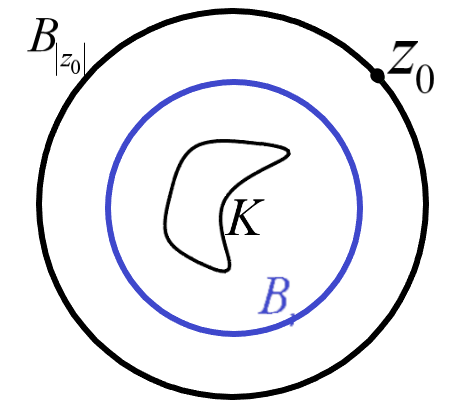
\includegraphics[width=3cm,height=2.7cm]{ch4_p3.png}
\end{wrapfigure}
由于$\displaystyle{\sum\limits_{n=0}^\infty a_nz_0^n}$收敛,故$\left|a_nz_0^n\right|\rightarrow0$
故存在$M\in\mathbb{R}.\ s.t.\ \left|a_nz_0^n\right|<M$\\
故当$z\in k$时,
$\displaystyle{\left|a_k\cdot a^k\right|=\left|a_n\cdot z_o^k\cdot \frac{z^k}{z_0^k}\right|\leqslant M\left(\left|\frac{z}{z_0}\right|\right)^k}$\\
由于$\displaystyle{\sum\limits_{n=0}^\infty\left|\frac{z}{z_0}\right|^n}$时收敛的,
故由\emph{Weierstrass}判别法得$\displaystyle{\sum\limits_{n=0}^\infty a_nz^n}$在$k$中一致收敛。\
%\\rightline{$\square$}
\end{proof}

\noindent 由定理\emph{4.2.3}以及\emph{Weierstrass}定理可以得到:

\begin{theorem}
    幂级数在其收敛圆内确定了一个全纯函数\par
    \qquad\quad\, 那么在收敛圆圆周上的收敛性如何呢?
\end{theorem}

\begin{eg}
    级数$\displaystyle{\sum\limits_{n=0}^\infty z^n}$的收敛半径为1,它在收敛圆周$|z|=1$上处处发散.
\end{eg}

\begin{eg}
    级数$\displaystyle{\sum\limits_{n=0}^\infty \frac{z^n}{n^2}}$的收敛半径为1,它在收敛圆周$|z|=1$上处处收敛.
\end{eg}

\begin{eg}
    级数$\displaystyle{\sum\limits_{n=0}^\infty \frac{z^n}{n}}$的收敛半径为1,
    它在收敛圆周$|z|=1$上在$z=e^{i\theta}(0<\theta<2\pi)$处收敛,在1处发散.
\end{eg}

\begin{proof}
    显然$z=1$时级数时发散的\\
    当$\theta\neq0$时$\displaystyle{\sum\limits_{n=0}^\infty\frac{z^n}{n}=
    \sum\limits_{n=0}^\infty\frac{\cos n\theta}{n}+i\cdot\sum\limits_{n=0}^\infty \frac{\sin n\theta}{n}}$
    由实数项级数的\emph{Dirichlet}判别法,\\
    得$\displaystyle{\sum\limits_{n=0}^\infty\frac{\cos n\theta}{n},\ \sum\limits_{n=0}^\infty \frac{\sin n\theta}{n}}$收敛\\
\end{proof}
由上述例子可知,收敛圆周上的收敛性无法确定\par 这也是我们下面要探讨的问题\par
设级数$\displaystyle{\sum\limits_{n=0}^\infty a_n(z-z_0)^n}$的收敛半径为$R$,
我们来研究$\displaystyle{\xi\in B(z_0,R),\sum\limits_{n=0}^\infty a_n(\xi-z_0)^n}$与和函数$f$的关系:
令$\displaystyle{\omega=\frac{z-z_0}{\xi-z_0}}$
故$\omega\in B(0,1)$,级数可改写为$\displaystyle{\sum\limits_{n=0}^\infty b_n\omega^n},b_n=a_n(\xi-z_0)^n$,
故新的幂级数的收敛半径为1,故以下我们在收敛半径为1的情况下做讨论.

\begin{theorem}[*]
    设$g$是定义在单位圆中的函数,$e^{i\theta_0}$是单位圆上的一点,记$S_\alpha(e^{i\theta_0})$为以$e^{i\theta_0}$为顶点,
    以$e^{i\theta_0}$点对应的极径在单位圆内侧向两侧张出的张角为$2\alpha$
    的角形区域$(\alpha<\frac{\pi}{2})$
\end{theorem}

%排的有问题
\begin{wrapfigure}[2]{r}{3cm}
    \centering
    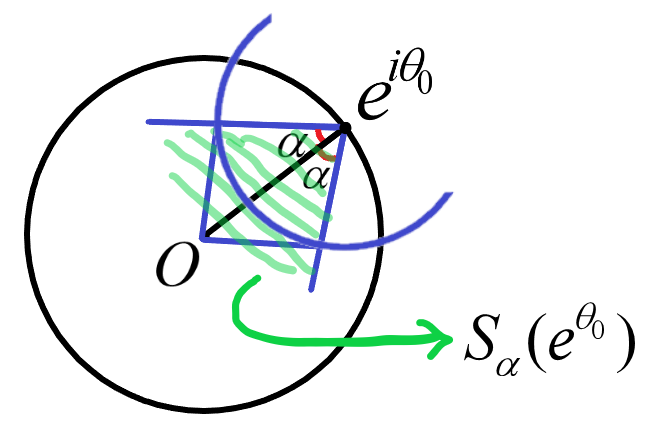
\includegraphics[width=3cm,height=2cm]{ch4_p4_1st.png}
\end{wrapfigure}
\noindent \emph{若$z$在$S_\alpha(e^{i\theta_0})$中趋于$e^{i\theta_0}$时$g(z)$有极限$C$则称$g$在$\theta_0$处有非切向极限$C$,记为
$\displaystyle{\lim\limits_{\substack{z\to e^{i\theta_0}\\z\in S_\alpha(e^{i\theta_0})}}g(z)=C}$}
\\
\\
\begin{theorem}[*](\rm \emph{Abel} \uppercase\expandafter{\romannumeral2})
    设$\displaystyle{f(z)=\sum\limits_{n=0}^\infty a_nz^n}$的收敛半径为$R=1$,
    且级数在$z=1$处收敛于$S$,则$f$在$z=1$处有非切向极限$S$
\end{theorem}
\noindent\emph{证明.}
记$\displaystyle{\sigma_{n,\rho}=\sum\limits_{i=1}^p a_{n+i}}$由条件得$\displaystyle{\sum\limits_{n=0}^\infty a_n}$收敛.\\
故$\forall\epsilon>0 ,\ \exists$正整数$N,\  s.t.\ $当$n>N$时,对任意自然数$p$有$|\sigma_{n,p}|<\epsilon$\\
由于
\begin{align*}
    \sum\limits_{i=1}^pa_{n+i}\cdot z^{n+i}&=\sum\limits_{i=1}^{p-1}(\sigma_{n,i+1}-\sigma_{n,i})z^{n+1+i}+\sigma_{n,1}z^{n+1}\\
    &=\sum\limits_{i+1}^{p-1}\sigma_{n,i}z^{n+i}\cdot(1-z)+\sigma_{n,p}z^{n+p}\\
    &=z^{n+1}(1-z)\cdot\sum\limits_{i=1}^{p-1}(\sigma_{n,i}\cdot z^{i-1})+\sigma_{n,p}\cdot z^{n+p}
\end{align*}
故当$|z|<1,n>N$.时有:$\displaystyle{\left|\sum\limits_{i=1}^pa_{n+i}\cdot z^{n+i}\right|
<\epsilon\cdot|1-z|\cdot\sum\limits_{n=p}^\infty|z^n|+\epsilon=\epsilon\left(\frac{|1-z|}{1-|z|}+1\right)}$\\
任取$\displaystyle{z\in S_\alpha(1)\cap B(1,\delta)}$记$|z|=r,|1-z|=\rho$则由余弦定理得$r^2=1+\rho-2\rho\cos\theta$\\
\begin{wrapfigure}[3]{r}{3cm}
    \centering
    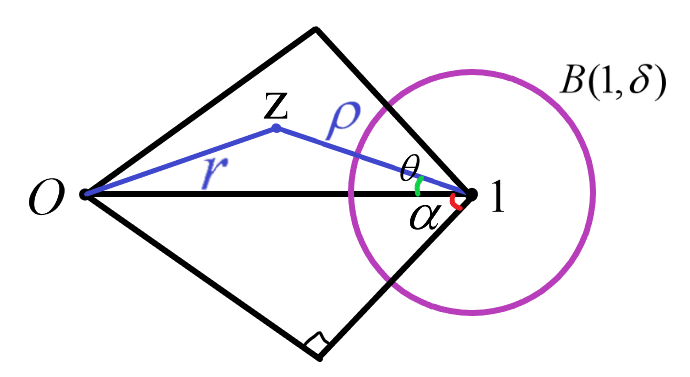
\includegraphics[width=3.5cm,height=2.0cm]{ch4_p4_2nd.png}
\end{wrapfigure}
故$\displaystyle{\frac{|1-z|}{1-|z|}=\frac{\rho}{1-r}=\frac{\rho(1+r)}{1-r^2}
\leqslant\frac{2\rho}{2\rho\cos\theta-\rho^2}=\frac{2}{2\cos\theta-\rho}}$\\
又由于$z\in B(1,\delta).$故$\rho<\delta<\cos\alpha<\cos\theta$故$\displaystyle{\frac{|1-z|}{1-|z|}<\frac{2}{\cos\alpha}}$\\
故$\displaystyle{\left|\sum\limits_{i=1}^pa_{n+i}\cdot z^{n+i}\right|<\epsilon(\frac{2}{\cos\alpha}+1)}$
,故$\displaystyle{\sum\limits_{n=0}^\infty a_nz^n}$在$\displaystyle{S_\alpha(1)\cap B(1,\delta)}$上一致收敛
设和函数为$f$,由一致收敛性得$f$在$\displaystyle{S_\alpha(1)\cap B(1,\delta)}$上连续,
故$\displaystyle{\lim\limits_{\substack{z\in S_\alpha(1)\\z\to 1}}f(z)=f(1)=S}$\\\rightline{$\square$}



%以下是p5-8
\begin{eg}
	\color{blue}计算级数$\displaystyle{\sum_{n=1}^{\infty} \frac{z^n}{n}}$的和.
	
	\color{black}
	显然收敛半径为1且和函数$\displaystyle{f(z) \in H(D)}$,故$\displaystyle{f(z)=\sum_{n=1}^{\infty} \frac{z^n}{n}}$, 得$\displaystyle{f'(z)=\sum_{n=1}^{\infty} z^{n-1} = \frac{1}{1-z}}$
	由此得$\displaystyle{f(z)=-log(1-z), \vert z \vert < 1}$.
	
	前面分析得在$\displaystyle{\vert z \vert = 1}$上除$\displaystyle{z=1}$均收敛,故由定理4.2.9得当$\displaystyle{z=e^{i\theta} (0 < \theta < 2\pi}$时,有:$\displaystyle{\sum_{n=1}^{\infty} \frac{e^{in\theta}}{n} = -log(1-e^{i\theta})=-log \vert 1 - e^{i\theta} \vert - i arg(1 - e^{i\theta})}$ (*).
	
	由几何关系得$\displaystyle{\vert 1 - e ^{i\theta} \vert = 2 \sin \frac{\theta}{2}, arg(1 - e^{i\theta}) = - \phi}$ 
	
	故由(*)式以及比较实虚部得$\displaystyle{\sum_{n=1}^{\infty} \frac{cos n\theta}{n} = -log(2 \sin \frac{\theta}{2})}$, $\displaystyle{\sum_{n=1}^{\infty} \frac{\sin n\theta}{n} = \frac{\pi - \theta} {2}}$
	
	特别地,$\displaystyle{\theta = \pi}$时得$\displaystyle{\sum_{n=1}^{\infty} \frac{(-1)^{n-1}}{n} = log 2}$; $\displaystyle{\theta = \pi / 2}$时得$\displaystyle{\sum_{k=0}^{\infty} \frac{(-1)^k}{2k+1} = \pi / 4}$.
\end{eg}

\section{解析函数的{\rm Taylor}展开}
\begin{theorem}
	\color{blue}
	(\rm Taylor) \color{black} (略)
\end{theorem}

\begin{proof}
	对于此定理有两种不同证法。详见史济怀《复变函数》及Stein 《 Complex Analysis》.
\end{proof}

\begin{theorem}
	由4.3.1以及4.2.4得$\displaystyle{f}$在$\displaystyle{z_0}$处解析的充要条件为$\displaystyle{f}$ 在$\displaystyle{z_0}$的邻域内可展为幂级数:$\displaystyle{f(z)=\sum_{n=0}^{\infty}a_n (z-z_0)^n}$.
\end{theorem}

\begin{theorem}
	$\displaystyle{z_0}$为$\displaystyle{f}$的$\displaystyle{m}$阶零点的充要条件是$\displaystyle{f}$在$\displaystyle{z_0}$的邻域内可写成$\displaystyle{f(z)=(z-z_0)^m g(z)}$。其中$\displaystyle{g}$在$\displaystyle{z_0}$处解析,且$\displaystyle{g(z_0) \neq 0}$.
\end{theorem}
\begin{proof}
	略.
\end{proof}

\begin{theorem}\color{blue}(零点独立性定理)
	\color{black}
	设$\displaystyle{D}$为$\displaystyle{\mathbb{C}}$中的域,$\displaystyle{f \in H(D)}$,若$\displaystyle{f \not\equiv 0}$,且$\displaystyle{f(a)=0}$,则存在$\displaystyle{\delta > 0}$, s.t. $\displaystyle{\forall z \in B(z_0, \delta) \\ \{z_0\}}$有$\displaystyle{f(z) \neq 0}$.
\end{theorem}
\begin{proof}
	略. 史济怀.方企勤.Stein给出了两种不同的证明方法.
\end{proof}


\begin{theorem}\color{blue}(唯一性定理)
	\color{black}
	设$\displaystyle{D}$为$\displaystyle{\mathbb{C}}$中的域,$\displaystyle{f_1,f_2 \in H(D)}$.若存在极限在$\displaystyle{D}$中的点列$\displaystyle{z_n}$ s.t. $\displaystyle{f_1(z_n) = f_2(z_n), n=1,2,...}$,则在$\displaystyle{D}$ 中有$\displaystyle{f_1 \equiv f_2}$.
	
\end{theorem}
\begin{proof}
	略.
\end{proof}


\begin{eg} 
	\color{blue} $\displaystyle{{\sin}^2 z + \cos^2 z \equiv 1, z \in \mathbb{C}}$
	\color{black}
\end{eg}
\begin{proof}
	取点列$\displaystyle{\{a_n\}}$:$\displaystyle{a_n = \frac{1}{n}}$,得$\displaystyle{a_n \rightarrow 0}$. 故由4.3.7得证.
\end{proof}

\begin{eg}
	\color{blue}
	证明:$\displaystyle{e^z =\sum_{n=0}^{\infty} \frac{z^n}{n!}, z \in \mathbb{C}}$
	\color{black}
\end{eg}
\begin{proof}
	由Stirling公式得,$\displaystyle{f(z)=\sum_{n=0}^{\infty} \frac{z^n}{n!}}$的收敛半径为 $\displaystyle{R=+\infty}$,显然$\displaystyle{e^z}$与$\displaystyle{f(z)}$均为整函数,且在实轴上相等,由4.3.7得证.
\end{proof}
利用这样的方法,我们可以将{\rm Taylor }公式从$\displaystyle{\mathbb{R}}$上扩张到$\displaystyle{\mathbb{C}}$上.

\section{{\rm Laurent } 级数}
\begin{theorem}({\rm Laurent}级数. 主要部分.)
	略.
\end{theorem}

\begin{theorem}
	\color{blue}
	({\rm Laurent})
	\color{black}
	若{\rm Laurent}级数的收敛域圆环$\displaystyle{D = \{z: r< \vert z - z_0 \vert < R \}}$,那么它在$\displaystyle{D}$中绝对收敛且内闭一致收敛,那么它的和函数在$\displaystyle{D}$中解析.
\end{theorem}

\begin{theorem}
	\color{blue}
	({\rm Laurent})
	\color{black}
	设$\displaystyle{D=\{z : r < \vert z \vert < R\}}$. 若$\displaystyle{f \in H(D)}$,则$\displaystyle{f}$在$\displaystyle{D }$中可以展为{\rm Laurent}级数,$\displaystyle{f(z)=\sum_{n = -\infty}^{\infty} a_n(z - z_0)^n}, z \in D$,其中$\displaystyle{a_n = \frac{1}{2\pi_i}  \int_{\gamma_\rho} \frac{f(\xi)} {(\xi - z_0)^{n+1}} \di \xi }$,其中$\displaystyle{\gamma_\rho = \{ \xi : \vert \xi - z_0 \vert  = \rho \} (r < \rho < R)}$,并且展开式唯一.
	
	这个定理是4.4.2的逆定理,证明略.
\end{theorem}


\begin{eg}
	\color{blue}
	$\displaystyle{f(z) = \frac{1}{\sin \frac{1}{z}}}$ 在以0为圆心的圆形去心邻域上是否可展为{\rm Laurent } 级数?
	\color{black}
\end{eg}
\begin{jie}
	
	取$\displaystyle{\{z_n\}, z_n = \frac{1}{n\pi}, n \in \mathbb{N} ^* \Rightarrow \sin \frac{1}{z_n} = 0}$. 故有一列趋于0的$\displaystyle{f}$的奇点. 故$\displaystyle{f}$ 在0的去心邻域内不可展为{\rm Laurent } 级数.
\end{jie}

\begin{eg}
	\color{blue}
	设$\displaystyle{f(z)=\frac{1}{(z-1)(z-2)}}$,设求在$\displaystyle{D_1 = \{ z : 1 < \vert z \vert < 2\}, D_2 = \{ z : 2 < \vert z \vert < + \infty}$上的{\rm Laurent} 展式.
	\color{black}
\end{eg}
\begin{jie}
	
	$\displaystyle{z \in D_1}$ 时,
	\begin{align*}
	\frac{1}{(z-1)(z-2)} &= \frac{1}{z-2} - \frac{1}{z-1} \\
	&= -\frac{1}{2} \frac{1}{1 - \frac{z}{2}} - \frac{1}{z} \frac{1}{1 - \frac{1}{z}}\\
	&= -\frac{1}{2} \sum_{n=0}^{\infty} (\frac{z}{2})^n - \frac{1}{z} \sum_{n=0}^{\infty} (\frac{1}{z})^n\\
	&=-\sum_{n=0}^{\infty} \frac{z^n}{z^{n+1}} - \sum_{n=1}^{\infty} \frac{1}{z^n}
	\end{align*}
	$\displaystyle{z \in D_2}$时,
	\begin{align*}
	\frac{1}{(z-1)(z-2)} &= \frac{1}{z-2} - \frac{1}{z-1} \\
	&= -\frac{1}{z} \frac{1}{1 - \frac{2}{z}} - \frac{1}{z} \frac{1}{1 - \frac{1}{z}}\\
	&= -\frac{1}{z}( \sum_{n=0}^{\infty} (\frac{2}{z})^n -\sum_{n=0}^{\infty} (\frac{1}{z})^n)\\
	&= \sum_{n=0}^{\infty} \frac{2^n - 1}{z^{n+1}}
	\end{align*}		
	
\end{jie}

\section{孤立奇点}
三种奇点:可去奇点、极点、本性奇点.
\begin{theorem}
	设$\displaystyle{a \in \mathbb{C}, f(z) \in H(B(a, R) \backslash \{ a\})}$则下列三个命题等价.
	\begin{enumerate} [(1)]
		\item $\displaystyle{a}$是$\displaystyle{f(z)}$的可去奇点.
		\item $\displaystyle{f(z)}$在$\displaystyle{B(a, \delta)}$上有界.
		\item $\displaystyle{f(z)}$在$\displaystyle{a}$处的{\rm Laurent} 展式的主部为0.
	\end{enumerate}
\end{theorem}

\begin{theorem}
	设$\displaystyle{a \in \mathbb{C}, f(z) \in H(B(a, R) \backslash \{ a\})}$则下列三个命题等价.
	\begin{enumerate} [(1)]
		\item $\displaystyle{a}$是$\displaystyle{f(z)}$的极点(m阶).
		\item $\displaystyle{f(z) = \frac{g(z)}{(z - a) ^ m}}$,其中$\displaystyle{m \in \mathbb{N}}$, $\displaystyle{g(z)}$在$\displaystyle{B(a, \delta)}$上解析且不为0$\displaystyle{(\delta \leq R)}$.
		\item $\displaystyle{f(z)}$的{\rm Laurent}展式中主部中只有有限多个系数不为0$\displaystyle{(\forall n > m, a_n = 0)}$.
		
	\end{enumerate}
\end{theorem}

\begin{theorem}
	设$\displaystyle{a \in \mathbb{C}, f \in H(B(a, R) \backslash \{a\})}$,则$\displaystyle{a}$是$\displaystyle{f}$的本性奇点的充要条件是$\displaystyle{f(z)}$的{\rm Laurent}展式主部中有无穷多项的系数不为0.
\end{theorem}
上述三个定理的证明详见方企勤《复变函数》.

\begin{theorem}
	\color{blue}
	(WeierStrass)
	\color{black}
	若$\displaystyle{a}$是$\displaystyle{f}$的一个本性奇点,则对于$\displaystyle{z=a}$的任一邻域$\displaystyle{B(a, \delta)}$,有$\displaystyle{f(B(a, \delta)) = \mathbb{C}}$.
\end{theorem}
\begin{proof}
	略.见笔记.
\end{proof}

\section{相关的其他结论以及习题列举}
\begin{theorem}
	\color{blue}
	(解析延拓定理).
	\color{black}
	设区域$\displaystyle{\Omega}$可被一条可求长曲线$\displaystyle{\gamma}$分为两个区域$\displaystyle{\Omega_1}$和$\displaystyle{\Omega_2}$,$\displaystyle{\Omega {\backslash} \gamma = \Omega_1 \cup \Omega_2, \Omega_1 \cap \Omega_2 = \emptyset}$.设$\displaystyle{f \in C(\Omega), f \in H(\Omega_i), i = 1,2}$,则$\displaystyle{f(z) \in H(\Omega)}$.
\end{theorem}
\begin{proof}
	任取$\displaystyle{\Omega}$上的一条曲线$\displaystyle{C}$,不妨设$\displaystyle{C \not\subset \Omega_1, C \not\subset \Omega_2}$,故$\displaystyle{\int_C f(z) \di z  = \int_{C_1} f(z) dz + \int_{C_2} f(z)dz}$.
	
	由定理3.2.4和{\rm Mereron}定理得证.
\end{proof}
注意与$Painlev\acute{e}$原理的区别.

\begin{theorem}
	\color{blue}
	(解析延拓定理).
	\color{black}
	设区域$\displaystyle{\Omega_j}$被一条可求长曲线$\displaystyle{\gamma}$分为两个区域$\displaystyle{\Omega_1}$和$\displaystyle{\Omega_2}$,$\displaystyle{\Omega {\backslash} \gamma = \Omega_1 \cup \Omega_2, \Omega_1 \cap \Omega_2 = \emptyset}$. 设$\displaystyle{f_i \in C(\Omega_i \cup \gamma) \cap H(\Omega_i), i=1,2, f_1(z) = f_2(z), z \in \gamma}$.
	设
	\begin{equation*}
	F(z) = \left\{
	\begin{aligned}
	f_1(z)& , & z \in \Omega_1 \cup \gamma \\ 
	f_2(z) & , & z \in \Omega_2
	\end{aligned}
	\right.
	\end{equation*}
	则$\displaystyle{F(z) \in H(\Omega)}$
\end{theorem}
\begin{proof}
	证明过程同4.6.1.
\end{proof}

\begin{theorem}
	\color{blue}
	({\rm Schwarz}反射原理)
	\color{black}
	设$\displaystyle{\Omega}$为$\displaystyle{\mathbb{C}}$上的区域,记$\displaystyle{I = \{ z: z \in \Omega, Imz = 0\}}$,且$\displaystyle{I \neq \emptyset}$. 记$\displaystyle{\Omega^+ = \{ z \in \Omega : Im z >0\} ,  \Omega^- = \{ \bar{z} : z \in \Omega^+ \}}$. 设$\displaystyle{f \in H(\Omega^+) \cap C(\Omega ^ + \cap I)}$且$\displaystyle{f(I) \subset \mathbb{R}}$,则存在$\displaystyle{F \in H(\Omega^+ \cup \Omega^- \cup I)}$, s.t. $\displaystyle{F(z) = f(z), z \in \Omega^+}$
\end{theorem}
\begin{proof}
	略. 见方企勤《复变函数》.
\end{proof}

\begin{theorem}
	设$\displaystyle{F(z, s) \in C(\Omega \times [0,1]) }$,$\displaystyle{\Omega}$为$\displaystyle{\mathbb{C}}$中开集,若$\displaystyle{F(z,s)}$对每个$\displaystyle{s}$,对$\displaystyle{z}$都是解析的,则定义在$\displaystyle{\Omega}$上的函数$\displaystyle{f(z):\overset{\Delta}{=} \int_0^1 F(z,s) \di s}$是解析的.
\end{theorem}
\begin{proof}
	略.见{\rm Stein} 即chb笔记.
\end{proof}

%以下是p.9-13
\begin{theorem}
	设$f \in f(\omega)$,$\omega$为开集,$k\in\omega$为紧集,则存在$\omega-k$中的有线条可求长$r_{1},r_{2}......r_{n}$,使得
	\begin{equation*}
	f(z)=\sum_{j=1}^{N}\frac{1}{2\pi i}\int_{r_{n}}\frac{f(\xi)}{\xi-z}\di{\xi}
	\end{equation*}
\end{theorem}
\begin{proof}
	设$d=c \cdot d(k,\omega^{c})$,其中$c$为常数且$0<c<\frac{1}{\sqrt{2}}$,考虑边平行于轴的边长为$d$的正方形组成的网格。
	故在$\Omega-K$中必定包含一个完整的方格,并且与$k$相交的方格不与$\Omega$相交。
	
	设$Q$为与$K$相交的方格的全集,由于$K$是紧集,故$Q$为有限集,设$Q={Q_{1},Q_{2}......Q_{n}}$
	我们取$r_{1},r_{2}......r_{n}$为$Q$中的方格中所有只属于唯一方格的方格边框。如图
	%@TODO:Here should be the figure%
	
	任取$K$中非方格边框的一点$z$,存在$1 \le j \le m , s.t.  z \in Q_{j},z\notin Q_{k} (k \ne j)$
	故由\emph{Cauchy}积分公式得
	
	\begin{equation*}
	f(z)=\int_{\partial Q_{k}}\frac{f(\xi)}{\xi - z}\di{\xi}=\delta_{n-j}\cdot f(z)
	\end{equation*}
	故
	\begin{equation*}
	f(z)=\sum_{k=1}^{m}\int_{\partial Q_{k}}\frac{f(\xi)}{\xi -z}\di{\xi}
	\end{equation*}
	
	而由于在对每个$Q_{k}$的边界进行线积分的时候,对于除去$r_{1},r_{2}......r_{n}$之外的$Q$中方格边框均正向反向各积分一次
	,故
	\begin{equation*}
	f(z)=\int_{r_{k}}\dfrac{f(\xi)}{\xi - z}\di{\xi}
	\end{equation*}
	而可得$r_{k} \in \Omega /k,k=1,2.....m$,显然$r_{1},r_{2}......r_{n}$首尾相连得到了一条$\Omega /k$中的可求长闭曲线        
\end{proof}

\begin{eg}
	\color{blue}设$G={z\in C,0<\arg z<\frac{\pi}{4}}$,设$f\in H(G)\cup C(\bar G)$。若$f$在实轴上区间$[a,b]$恒为$0$,则$f(x)\equiv 0,x\in G$
	
	\color{black}
	\begin{proof}
		在$[a,b]$下方做延拓(如图),
		%@TODO:A figure here%
		
		有$\partial G \cap \partial D=[a,b]$。做$f_{1}:D\cup [a,b] \to {0} ,f_{1}(z)\equiv 0,z\in D\cup [a,b]$。
		故$\forall z\in [a,b]$有$f_{1}(z)=f(z)=0$。记$G\cup D \cup [a,b]=M$,故由解析延拓定理得存在$F(z)\in H(M)$
		且$f_{1}(z)=F(z),z\in D\cup [a,b],F(z)=f(z),z\in G$,显然存在一个M中的点列${Z_{n}}$,且有极限点$a\in M^{o}$,
		并且$F(Z_{n})=0。\forall n\in N。$由零点孤立性定理得$f(z)\equiv 0,z\in M$,故$f(z)\equiv 0,z\in G$
		
		类似于上一例题的推理过程,对于区域G,设$f\in H(G)\cap C(\bar{G})$,若存在一条可求长连续曲线$r \in \partial G$,
		有$f(z)\equiv 0,z\in r$,并且可以在r的异于G一侧做一区域E,使得$r\in \partial E$,且$E\cap G=\phi$,完全与上一例题中的过程相同可得$f(z)\equiv 0,\forall z\in G$
	\end{proof}
\end{eg}
\begin{eg}
	\color{blue}设$f_{n}(z)\in H(D)$,D为中区域,$\sum_{n=1}^{\infty}|f_{n}(z)|$在$D$内一致收敛,证明:$\sum_{n=1}^{\infty}|f_{n}(z)|$在D内内闭一致收敛。
	
	\color{black}
	\begin{proof}
		任取$D$中的紧集$K$,设$d=d(\partial D,k)$,记$\rho=\frac{d}{2}$
		
		故$z\in k$时
		\begin{equation*}
		\sum\limits_{i=1}^{n}\left|f'_{n+i}(z)\right|=\sum\limits_{i=1}^{p}\left|\int_{|\xi -z|=\rho }\dfrac{f_{i}(\xi)\di{\xi}}{(\xi -z)^{2}}\right|\cdot \dfrac{1}{2\pi}
		\end{equation*}
		\begin{equation*}
		\le \int_{|\xi -z|=\rho }\frac{\sum_{i=1}^{p}|f_{i}(\xi)|}{|(\xi -z)^{2}|}|\di{\xi}|\cdot \dfrac{1}{2\pi}\le \dfrac{\epsilon}{\rho}
		\end{equation*}
	\end{proof}
\end{eg}
\begin{eg}
	\color{blue}写出$e^{\frac{1}{1-z}}$,在$|z|<1$和$1<z<+ \infty$的部分\emph{Laurent}展式
	
	\color{black}设$f(z)=e^{z}$,显然$f$为常    函数,故$f(z)=\sum_{n=0}^{\infty}\frac{z^{n}}{n!}$,可以利用4.3.7将R上的展开到 D上
	可得$f(\frac{1}{1-z})=\sum\limits_{n=0}^{\infty}\frac{1}{n!}(\frac{1}{1-z})^{n}$,当$|z|<1$时,有如下错误解法。
	\begin{jie}{(错误)}
		\begin{equation*}
		\frac{1}{1-z}=\sum_{n=0}^{\infty}z^{n}=1+z+z^{2}+o|z|^{2} 
		\end{equation*}
		\begin{equation*}
		\Rightarrow f(\frac{1}{1-z})=1+\frac{1}{1-z}+\frac{1}{2}(\frac{1}{1-z})^{2}+...\dots
		\end{equation*}
		做到这里你就发现做不下去了,为什么?因为$(\frac{1}{1-z})^{n}=1+o(|z|)$
	\end{jie}
	\begin{jie}{(正确)}
		考虑展开$e^{\frac{z}{1-z}}$
		\begin{equation*}
		\dfrac{z}{1-z}=\sum\limits_{n=1}^{\infty}z^{n}=z+z^{2}+o|z|^{2} =o(1)
		\end{equation*}
		\begin{equation*}
		\Rightarrow f(\dfrac{z}{1-z})=1+\dfrac{z}{1-z}+\dfrac{1}{2}(\dfrac{z}{1-z})^{2})+o|z|^{2}
		\end{equation*}
		\begin{equation*}
		=1+(z+z^{2}+o|z|^{2})+\frac{1}{2}(z+z^{2}+o|z|^{2})^{2}+o|z|^{2}
		\end{equation*}
		\begin{equation*}
		=1+z+\dfrac{3}{2}z^{2}+o|z|^{2}
		\end{equation*}
		\begin{equation*}
		\Rightarrow e^{\dfrac{1}{1-z}}=e+ez+\dfrac{3e}{2}z^{2}+o|z|^{2}
		\end{equation*}
	\end{jie}
	当$1<|z|<+\infty$时,同上述讨论。
\end{eg}
\begin{eg}
	\color{blue}若$f(z)$在$0<|z-a|<R$上解析,$f$不为常值函数,且圆环上有一列点$z_{n}\rightarrow a$,有$f(z_{n})=0$。证明:$a$为$f(z)$的本性奇点。
	
	\color{black}
	\begin{proof}
		若$a$为可去奇点,则$\displaystyle\lim_{z\rightarrow a}f(z)$存在,故$\displaystyle\lim_{z\rightarrow a}f(z)=0$,补充定义$f(a)=0$故$f$在$|z-a|<R$上解析。由零点孤立性定理得$f(z)\equiv 0 , 0\le |z-a|<R$矛盾,
		
		若$a$为极点,故$\displaystyle\lim_{z\rightarrow a}f(z)=+\infty$,而$\displaystyle\lim_{n\rightarrow \infty}f(z_{n})=0$矛盾!
	\end{proof}	
\end{eg}
\begin{eg}
	\color{blue}设$f(z)$在圆环$0<r<|z-a|<R<+\infty$内解析,在闭圆环$r\le |z-a|\le R$上连续,且$f(Re^{i\Theta} )=0,(0\le \theta \le 2\pi)$。证明:$f(z)\equiv 0,(r<|z-a|<R)$
	\color{black}
	\begin{jie}{1}
		
		
		设$F(z)=f(\frac{r^{2}}{\bar{z}}),z\in \{z|\frac{r^{2}}{R} \le |z-a|\le r\}$,显然,$F(z)$在$\{z|\frac{r^{2}}{R} < |z-a|< r\}$
		上解析,在$\{z|\frac{r^{2}}{R} \le |z-a|< r\}$上连续。并且当$|z|=r$时,$F(z)=f(\frac{r^{2}}{\bar{z}})=f(z)$。$|z|=\frac{r^{2}}{R}$时,$F(z)=0$.
		
		设$D=\{z|\frac{r^{2}}{R} \le |z-a| < r\}$,故由解析延拓定理得存在$F_{1}\in H(D)\cap C(\bar{D})$。并且$F_{1}(z)=F(z),z\in \{z|\frac{r^{2}}{R} \le |z-a|\le r\}$,且$F_{1}(z)=f(z),z\in \{z|\frac{r^{2}}{R} \le |z-a|\le r\}$。
		
		又由于$\partial D =\{ z:|z|=\frac{r^{2}}{R} $或$R\}$。$\Rightarrow \forall z \in \partial D$有$F_{1}(D)=0$故最大模存理$F_{1}(z)\equiv 0 ,z\in \bar{D}$故$f(z)\equiv 0.(r<|z-a|<R)$
	\end{jie}
	\begin{jie}{2}
		
		
		同4.6.5第一个例子
	\end{jie}
\end{eg}
\begin{eg}
	\color{blue}若$f\in H(\{ z:0<|z-a|<k\}  )$且$\displaystyle\lim_{z \rightarrow a}(z-a)f(z)=0$。证明:$a$是$f(z)$的可去奇点。
	
	\color{black}
	\begin{proof}
		显然$a$是$g(z)=(z-a)f(z)$的可去奇点。利用定理4.5.1,再直接讨论\emph{Laurent}级数的系数即可
	\end{proof}
	
\end{eg}
\begin{eg}
	\color{blue}若$f$为整函数,并且$\infty$为$f$的可去奇点,证明$f$为常值函数。
	
	\color{black}
	\begin{proof}
		由定理4.5.1得$f$在$\infty$处的\emph{Laurent}展开式中幂次大于0的系数均为0。
		又由于$f$为整函数,故$f(z)$为常数。
	\end{proof}
\end{eg}
\begin{eg}
	\color{blue}设$f\in H(B(a,R )|\{ a\})$,且不为常值函数。记$u(z)=Ref(z)$,若$u(z)$有界,则$a$是$f$的可去奇点。
	\color{black}
	\begin{jie}{1}
		
		
		由\emph{Laurent}级数系数公式得$1\le n$时,$G_{n}=\frac{1}{2\pi i}\int_{|z-a|=\rho}f(z)(z-a)^{n-1}\di{z} \quad(0<\rho<R)$
		
		另一方面
		\begin{align*}
		G_{n}&=\frac{1}{2\pi i}\int_{|z-a|=\rho}f(z)(z-a)^{n-1}\di{z} \quad(0<\rho<R)\\
		&=\frac{1}{2\pi i}\int_{|z-a|=\rho}(\sum_{k=-\infty}^{\infty }\overline{C_{k}}\cdot\overline{(z-a)^{k}})(z-a)^{n-1}\di{z} \quad(0<\rho<R)\\
		&=\frac{1}{2\pi i}\int_{|z-a|=\rho}\sum_{k=-\infty}^{\infty }\overline{C_{k}} \cdot \rho^{n+k-1}(\frac{z-a}{|z-a|})^{n-1}\di{z} \quad(0<\rho<R)\\
		&=\frac{1}{2\pi}\sum_{k=-\infty}^{+\infty}\overline{C_{k}}\int_{0}^{2\pi}\rho^{k+n}e^{i(n-k)\theta}\di{\theta}=\overline{C_{n}}\rho^{2n}
		\end{align*}
		
		故我们可得$C_{-n}+\overline{C_{n}}\rho^{2n}=\frac{1}{\pi i}\int_{|z-a|=\rho}u(z)(z-a)^{n-1}\di{z}$
		
		故$|C_{-n}+\overline{C_{n}}\rho^{2n}|\le \frac{1}{\pi}|\int_{|z-a|=\rho}u(z)(z-a)^{n-1}\di{z}|<\frac{2\pi \rho}{\pi}\cdot M \cdot \rho^{n-1}=2M\rho^{n}(1\le n)$
		
		当$\rho\rightarrow 0$。得$C_{-n}=0(1\le n)$。故$a$为$f(z)$可去奇点。
	\end{jie}
	\begin{jie}{2}
		
		
		设$F(z)=e^{f(z)}$,故$F(z)$在$B(a,R)\{ a\}$上有界。故$|F(z)=e^{u(z)}\le e^{M}|$。故由定理4.5.1得。$a$为$F(z)$的可去奇点,补充定义$F(a)$使得$F(z)\in H(B(a,R))$
		
		又有$|F(z)|=e^{u(z)}\ge e^{-M}>0$。故在$a$的邻域内对数函数可取出单值解析分支。故$a$是$f(z)=\lg F(z)$的可去奇点。
	\end{jie}
	\begin{jie}{3}
		
		记$F(z)=\frac{f(z)}{f(z)-2M}$。故在$B(a,R)\{a\}$上有$|F(z)|\le 1$
		故$a$是$F(z)$的可去奇点。补充定义$F(a)$使得$F(z)\in H(B(a,R))$。
		
		由最大模原理得$|F(a)|<1$。而可解出$f(z)=\frac{2MF(z)}{1-F(z)}$。故由表达式得$\displaystyle\lim_{z\rightarrow a}f(z)$存在。故$a$为$f(z)$的可去奇点。
	\end{jie}
\end{eg}




%以下是p.9-13
\begin{theorem}
	设$f \in f(\omega)$,$\omega$为开集,$k\in\omega$为紧集,则存在$\omega-k$中的有线条可求长$r_{1},r_{2}......r_{n}$,使得
	\begin{equation*}
	f(z)=\sum_{j=1}^{N}\frac{1}{2\pi i}\int_{r_{n}}\frac{f(\xi)}{\xi-z}\di{\xi}
	\end{equation*}
\end{theorem}
\begin{proof}
	设$d=c \cdot d(k,\omega^{c})$,其中$c$为常数且$0<c<\frac{1}{\sqrt{2}}$,考虑边平行于轴的边长为$d$的正方形组成的网格。
	故在$\Omega-K$中必定包含一个完整的方格,并且与$k$相交的方格不与$\Omega$相交。
	
	设$Q$为与$K$相交的方格的全集,由于$K$是紧集,故$Q$为有限集,设$Q={Q_{1},Q_{2}......Q_{n}}$
	我们取$r_{1},r_{2}......r_{n}$为$Q$中的方格中所有只属于唯一方格的方格边框。如图
	%@TODO:Here should be the figure%
	
	任取$K$中非方格边框的一点$z$,存在$1 \le j \le m , s.t.  z \in Q_{j},z\notin Q_{k} (k \ne j)$
	故由\emph{Cauchy}积分公式得
	
	\begin{equation*}
	f(z)=\int_{\partial Q_{k}}\frac{f(\xi)}{\xi - z}\di{\xi}=\delta_{n-j}\cdot f(z)
	\end{equation*}
	故
	\begin{equation*}
	f(z)=\sum_{k=1}^{m}\int_{\partial Q_{k}}\frac{f(\xi)}{\xi -z}\di{\xi}
	\end{equation*}
	
	而由于在对每个$Q_{k}$的边界进行线积分的时候,对于除去$r_{1},r_{2}......r_{n}$之外的$Q$中方格边框均正向反向各积分一次
	,故
	\begin{equation*}
	f(z)=\int_{r_{k}}\dfrac{f(\xi)}{\xi - z}\di{\xi}
	\end{equation*}
	而可得$r_{k} \in \Omega /k,k=1,2.....m$,显然$r_{1},r_{2}......r_{n}$首尾相连得到了一条$\Omega /k$中的可求长闭曲线        
\end{proof}

\begin{eg}
	\color{blue}设$G={z\in C,0<\arg z<\frac{\pi}{4}}$,设$f\in H(G)\cup C(\bar G)$。若$f$在实轴上区间$[a,b]$恒为$0$,则$f(x)\equiv 0,x\in G$
	
	\color{black}
	\begin{proof}
	在$[a,b]$下方做延拓(如图),
	%@TODO:A figure here%
	
	有$\partial G \cap \partial D=[a,b]$。做$f_{1}:D\cup [a,b] \to {0} ,f_{1}(z)\equiv 0,z\in D\cup [a,b]$。
	故$\forall z\in [a,b]$有$f_{1}(z)=f(z)=0$。记$G\cup D \cup [a,b]=M$,故由解析延拓定理得存在$F(z)\in H(M)$
	且$f_{1}(z)=F(z),z\in D\cup [a,b],F(z)=f(z),z\in G$,显然存在一个M中的点列${Z_{n}}$,且有极限点$a\in M^{o}$,
	并且$F(Z_{n})=0。\forall n\in N。$由零点孤立性定理得$f(z)\equiv 0,z\in M$,故$f(z)\equiv 0,z\in G$
	
	类似于上一例题的推理过程,对于区域G,设$f\in H(G)\cap C(\bar{G})$,若存在一条可求长连续曲线$r \in \partial G$,
	有$f(z)\equiv 0,z\in r$,并且可以在r的异于G一侧做一区域E,使得$r\in \partial E$,且$E\cap G=\phi$,完全与上一例题中的过程相同可得$f(z)\equiv 0,\forall z\in G$
	\end{proof}
\end{eg}
\begin{eg}
	\color{blue}设$f_{n}(z)\in H(D)$,D为中区域,$\sum_{n=1}^{\infty}|f_{n}(z)|$在$D$内一致收敛,证明:$\sum_{n=1}^{\infty}|f_{n}(z)|$在D内内闭一致收敛。
	
	\color{black}
	\begin{proof}
	任取$D$中的紧集$K$,设$d=d(\partial D,k)$,记$\rho=\frac{d}{2}$
	
	故$z\in k$时
	\begin{equation*}
	\sum\limits_{i=1}^{n}\left|f'_{n+i}(z)\right|=\sum\limits_{i=1}^{p}\left|\int_{|\xi -z|=\rho }\dfrac{f_{i}(\xi)\di{\xi}}{(\xi -z)^{2}}\right|\cdot \dfrac{1}{2\pi}
	\end{equation*}
	\begin{equation*}
	\le \int_{|\xi -z|=\rho }\frac{\sum_{i=1}^{p}|f_{i}(\xi)|}{|(\xi -z)^{2}|}|\di{\xi}|\cdot \dfrac{1}{2\pi}\le \dfrac{\epsilon}{\rho}
	\end{equation*}
	\end{proof}
\end{eg}
\begin{eg}
	\color{blue}写出$e^{\frac{1}{1-z}}$,在$|z|<1$和$1<z<+ \infty$的部分\emph{Laurent}展式
	
	\color{black}设$f(z)=e^{z}$,显然$f$为常    函数,故$f(z)=\sum_{n=0}^{\infty}\frac{z^{n}}{n!}$,可以利用4.3.7将R上的展开到 D上
	可得$f(\frac{1}{1-z})=\sum\limits_{n=0}^{\infty}\frac{1}{n!}(\frac{1}{1-z})^{n}$,当$|z|<1$时,有如下错误解法。
	\begin{jie}{(错误)}
		\begin{equation*}
		\frac{1}{1-z}=\sum_{n=0}^{\infty}z^{n}=1+z+z^{2}+o|z|^{2} 
		\end{equation*}
		\begin{equation*}
		\Rightarrow f(\frac{1}{1-z})=1+\frac{1}{1-z}+\frac{1}{2}(\frac{1}{1-z})^{2}+...\dots
		\end{equation*}
		做到这里你就发现做不下去了,为什么?因为$(\frac{1}{1-z})^{n}=1+o(|z|)$
	\end{jie}
	\begin{jie}{(正确)}
		考虑展开$e^{\frac{z}{1-z}}$
		\begin{equation*}
		\dfrac{z}{1-z}=\sum\limits_{n=1}^{\infty}z^{n}=z+z^{2}+o|z|^{2} =o(1)
		\end{equation*}
		\begin{equation*}
		\Rightarrow f(\dfrac{z}{1-z})=1+\dfrac{z}{1-z}+\dfrac{1}{2}(\dfrac{z}{1-z})^{2})+o|z|^{2}
		\end{equation*}
		\begin{equation*}
		=1+(z+z^{2}+o|z|^{2})+\frac{1}{2}(z+z^{2}+o|z|^{2})^{2}+o|z|^{2}
		\end{equation*}
		\begin{equation*}
		=1+z+\dfrac{3}{2}z^{2}+o|z|^{2}
		\end{equation*}
		\begin{equation*}
		\Rightarrow e^{\dfrac{1}{1-z}}=e+ez+\dfrac{3e}{2}z^{2}+o|z|^{2}
		\end{equation*}
	\end{jie}
	当$1<|z|<+\infty$时,同上述讨论。
\end{eg}
\begin{eg}
	\color{blue}若$f(z)$在$0<|z-a|<R$上解析,$f$不为常值函数,且圆环上有一列点$z_{n}\rightarrow a$,有$f(z_{n})=0$。证明:$a$为$f(z)$的本性奇点。
	
	\color{black}
	\begin{proof}
	若$a$为可去奇点,则$\displaystyle\lim_{z\rightarrow a}f(z)$存在,故$\displaystyle\lim_{z\rightarrow a}f(z)=0$,补充定义$f(a)=0$故$f$在$|z-a|<R$上解析。由零点孤立性定理得$f(z)\equiv 0 , 0\le |z-a|<R$矛盾,
	
	若$a$为极点,故$\displaystyle\lim_{z\rightarrow a}f(z)=+\infty$,而$\displaystyle\lim_{n\rightarrow \infty}f(z_{n})=0$矛盾!
	\end{proof}	
\end{eg}
\begin{eg}
	\color{blue}设$f(z)$在圆环$0<r<|z-a|<R<+\infty$内解析,在闭圆环$r\le |z-a|\le R$上连续,且$f(Re^{i\Theta} )=0,(0\le \theta \le 2\pi)$。证明:$f(z)\equiv 0,(r<|z-a|<R)$
	\color{black}
	\begin{jie}{1}
		
		
		设$F(z)=f(\frac{r^{2}}{\bar{z}}),z\in \{z|\frac{r^{2}}{R} \le |z-a|\le r\}$,显然,$F(z)$在$\{z|\frac{r^{2}}{R} < |z-a|< r\}$
		上解析,在$\{z|\frac{r^{2}}{R} \le |z-a|< r\}$上连续。并且当$|z|=r$时,$F(z)=f(\frac{r^{2}}{\bar{z}})=f(z)$。$|z|=\frac{r^{2}}{R}$时,$F(z)=0$.
		
		设$D=\{z|\frac{r^{2}}{R} \le |z-a| < r\}$,故由解析延拓定理得存在$F_{1}\in H(D)\cap C(\bar{D})$。并且$F_{1}(z)=F(z),z\in \{z|\frac{r^{2}}{R} \le |z-a|\le r\}$,且$F_{1}(z)=f(z),z\in \{z|\frac{r^{2}}{R} \le |z-a|\le r\}$。
		
		又由于$\partial D =\{ z:|z|=\frac{r^{2}}{R} $或$R\}$。$\Rightarrow \forall z \in \partial D$有$F_{1}(D)=0$故最大模存理$F_{1}(z)\equiv 0 ,z\in \bar{D}$故$f(z)\equiv 0.(r<|z-a|<R)$
	\end{jie}
	\begin{jie}{2}
		
		
		同4.6.5第一个例子
	\end{jie}
\end{eg}
\begin{eg}
	\color{blue}若$f\in H(\{ z:0<|z-a|<k\}  )$且$\displaystyle\lim_{z \rightarrow a}(z-a)f(z)=0$。证明:$a$是$f(z)$的可去奇点。
	
	\color{black}
	\begin{proof}
	显然$a$是$g(z)=(z-a)f(z)$的可去奇点。利用定理4.5.1,再直接讨论\emph{Laurent}级数的系数即可
	\end{proof}

\end{eg}
\begin{eg}
	\color{blue}若$f$为整函数,并且$\infty$为$f$的可去奇点,证明$f$为常值函数。
	
	\color{black}
	\begin{proof}
	由定理4.5.1得$f$在$\infty$处的\emph{Laurent}展开式中幂次大于0的系数均为0。
	又由于$f$为整函数,故$f(z)$为常数。
	\end{proof}
\end{eg}
\begin{eg}
	\color{blue}设$f\in H(B(a,R )|\{ a\})$,且不为常值函数。记$u(z)=Ref(z)$,若$u(z)$有界,则$a$是$f$的可去奇点。
	\color{black}
	\begin{jie}{1}
		
		
		由\emph{Laurent}级数系数公式得$1\le n$时,$G_{n}=\frac{1}{2\pi i}\int_{|z-a|=\rho}f(z)(z-a)^{n-1}\di{z} \quad(0<\rho<R)$
		
		另一方面
		\begin{align*}
		G_{n}&=\frac{1}{2\pi i}\int_{|z-a|=\rho}f(z)(z-a)^{n-1}\di{z} \quad(0<\rho<R)\\
		&=\frac{1}{2\pi i}\int_{|z-a|=\rho}(\sum_{k=-\infty}^{\infty }\overline{C_{k}}\cdot\overline{(z-a)^{k}})(z-a)^{n-1}\di{z} \quad(0<\rho<R)\\
		&=\frac{1}{2\pi i}\int_{|z-a|=\rho}\sum_{k=-\infty}^{\infty }\overline{C_{k}} \cdot \rho^{n+k-1}(\frac{z-a}{|z-a|})^{n-1}\di{z} \quad(0<\rho<R)\\
		&=\frac{1}{2\pi}\sum_{k=-\infty}^{+\infty}\overline{C_{k}}\int_{0}^{2\pi}\rho^{k+n}e^{i(n-k)\theta}\di{\theta}=\overline{C_{n}}\rho^{2n}
		\end{align*}
		
		故我们可得$C_{-n}+\overline{C_{n}}\rho^{2n}=\frac{1}{\pi i}\int_{|z-a|=\rho}u(z)(z-a)^{n-1}\di{z}$
		
		故$|C_{-n}+\overline{C_{n}}\rho^{2n}|\le \frac{1}{\pi}|\int_{|z-a|=\rho}u(z)(z-a)^{n-1}\di{z}|<\frac{2\pi \rho}{\pi}\cdot M \cdot \rho^{n-1}=2M\rho^{n}(1\le n)$
		
		当$\rho\rightarrow 0$。得$C_{-n}=0(1\le n)$。故$a$为$f(z)$可去奇点。
	\end{jie}
	\begin{jie}{2}
		
		
		设$F(z)=e^{f(z)}$,故$F(z)$在$B(a,R)\{ a\}$上有界。故$|F(z)=e^{u(z)}\le e^{M}|$。故由定理4.5.1得。$a$为$F(z)$的可去奇点,补充定义$F(a)$使得$F(z)\in H(B(a,R))$
		
		又有$|F(z)|=e^{u(z)}\ge e^{-M}>0$。故在$a$的邻域内对数函数可取出单值解析分支。故$a$是$f(z)=\lg F(z)$的可去奇点。
	\end{jie}
	\begin{jie}{3}
			
		记$F(z)=\frac{f(z)}{f(z)-2M}$。故在$B(a,R)\{a\}$上有$|F(z)|\le 1$
		故$a$是$F(z)$的可去奇点。补充定义$F(a)$使得$F(z)\in H(B(a,R))$。
		
		由最大模原理得$|F(a)|<1$。而可解出$f(z)=\frac{2MF(z)}{1-F(z)}$。故由表达式得$\displaystyle\lim_{z\rightarrow a}f(z)$存在。故$a$为$f(z)$的可去奇点。
	\end{jie}
\end{eg}

\chapter{微分与不定积分}
\section{第一组}
\exercise{1}设$E$是$\R{R}{\ }$中的一族区间的并集,试证$E$是可测集.
\begin{proof}
	设$E=\bigcup\limits_{\alpha\in \mathscr{A}}I_{\alpha}$,其中$ I_{\alpha} $为开区间或闭区间或半开闭区间,不妨设$m(E)<+\infty$,令$\mathscr{B}=\{I\subset\R{R}{\ }:I$是某个$I_{\alpha}$中的区间$\}$,故$\mathscr{B}$是$E$的一个Vitali覆盖,由Vitali定理得存在不交的区间列$\{I_k\},\ s.t.\ m\left( E\setminus \bigcup\limits_{k=1}^{\infty}I_k\right) =0$.设$I_k\subset I_{\alpha_k}$,故$$E=\left( E\setminus \bigcup_{k=1}^{\infty}I_k\right) \cup \left( \bigcup_{k=1}^{\infty}I_{\alpha_k}\right),\quad\alpha_k\in \mathscr{A} $$故E可测
\end{proof}


\exercise{2}设$\{x_n\}\subset [a,b]$,试做$[a,b]$上的递增函数,使得其不连续点 恰为$\{x_n\}$
\begin{proof}
	记\[f_n(x)=
	\begin{cases}
	\frac{1}{2^n}&x\geq x_n\\
	0&x< x_n\\
	\end{cases}\]
	$\qquad$由于$f_n(x)$是单调递增的,且函数项级数$\sum\limits\limits_{k=1}^{n}f_k(x)$关于n一致有上界2,故由定义式显然得到,函数项级数$\sum\limits\limits_{n=1}^{\infty}f_n(x)$是一致收敛的,且和函数存在,记为$f(x)$,故$f(x)\leq2$.\par 由一致连续性显然得到$f(x)$在除去$\{x_n\}$之外的点是连续的。令$g(x)=f(x),x\in [a,b]\setminus\bigcup\limits_{k=1}^{\infty}\{x_k\},$而$g(x)$在$x_n$处的取值我们可以根据$g(x)$在$[a,b]\setminus\bigcup\limits_{k=1}^{\infty}\{x_k\}$上的函数值进行定义,使得$g(x)$在$x_n$处是右连续的,故$g(x)$为递增函数。请读者自行证明$g(x)$在$x_n$处不是左连续的。故我们构造的$g(x)$即为满足要求的函数。
\end{proof}



\exercise{3}设$f(x)$是$(a,b)$上的递增函数,$E \subset(a,b)$,若对任给$\epsilon>0$,存在$(a_i,b_i)\subset (a,b)\ (i=1,2,....)$,使得$$\bigcup_i (a_i,b_i)\supset E ,\quad \sum\limits_i [f(b_i)-f(a_i)]<\epsilon,$$试证明$f'(x)=0\quad a.e.\ x \in E$
\begin{proof}
	记$E_{\alpha}^{(i)}$为$(a_i,b_i)$中所有开区间构成的开区间族,记$E_{\alpha}^{(i)}=\{I_{\alpha}^{(i)}:\alpha\in \mathscr{A}_i\}$,其中$I_{\alpha}^{(i)}$为开区间,故$\bigcup\limits_{i=1}^{+\infty}\bigcup\limits_{\alpha\in \mathscr{A}_i}I_{\alpha}^{(i)}$是E的Vitali覆盖。由Vitali定理,存在两两不交的子开区间列$\{I_k\}, \ s.t.\ \{I_k\}$满足$m(E\setminus \bigcup\limits_{k=1}^{\infty}I_k)=0$。由$I_k$的选取方式知存在唯一的i使得,$I_k\in E_{\alpha}^{(i)}$,记$I_k=(c_k,d_k)$,故由单调性得$$\sum\limits_{k=1}^{+\infty}\left(f(d_k)-f(c_k) \right)\leq\sum\limits_i\left(f(b_i)-f(a_i) \right)<\epsilon  $$
	故由Lebesgue定理得$$\int_E f'(x)\di{x}=\int_{\bigcup\limits_{k=1}^{+\infty}I_k}f'(x)\di{x}\ \leq\ \sum\limits_{k=1}^{\infty}\int_{I_k}f'(x)\di{x}\ \leq\ \sum\limits_{k=1}^{\infty}\left(f(d_k)-f(c_k) \right) \ <\ \epsilon$$
\end{proof}

\exercise{4}设$f(x)$在$[0,a]$上是有界变差函数,试证明函数$$F(x)=\frac{1}{x}\int_{0}^{x}f(t)\di{t}\quad,F(0)=0$$是$[0,a]$上的有界变差函数。
\begin{proof}
	由于f是有界变差函数,故由Jordan分解定理,$f(x)=g(x)-h(x)$,其中$g(x)$和$h(x)$为递增函数。故$F(x)=\displaystyle{\frac{1}{x}\int_{0}^{x}f(t)\di{t}}=\frac{1}{x}\displaystyle{\int_{0}^{x}g(t)\di{t}}-\displaystyle{\frac{1}{x}\int_{0}^{x}h(t)\di{t}}.$设$G(x)=\displaystyle{\frac{1}{x}\int_{0}^{x}g(t)\di{t}}$,$H(x)=\displaystyle{\frac{1}{x}\int_{0}^{x}h(t)\di{t}}.$设$h>0$,则:
	\[\begin{split}
	G(x+h)-G(x)&=\frac{1}{x+h}\int_{0}^{x+h}g(t)\di{t}-\frac{1}{x}\int_{0}^{x}g(t)\di{t}\\&=\frac{-h}{x(x+h)}\int_{0}^{x}g(t)\di{t}+\frac{1}{x+h}\int_{x}^{x+h}g(t)\di{t}\\&\geq\frac{h}{x+h}g(x)-\frac{h}{x(x+h)}\int_{0}^{x}g(t)\di{t}\\&=\frac{h}{x(x+h)}\int_{0}^{x}\left( g(x)-g(t)\right) \di{t}\geq 0
	\end{split}\]
	$\qquad$故$G(x)$是递增的,同理$H(x)$是递增的,故由Jordan分解定理得$F(x)$是有界变差函数。
\end{proof}



\exercise{5}设$\{f_k(x)\}$是$[a,b]$上的有界变差函数列,且有$$\bigvee\limits_a^b(f_k)\leq M \quad (k=1,2,...)\ \ ;\ \ \li{k\to\infty}f_k(x)=f(x),\quad x\in[a,b]$$试证明$f\in BV([a,b]),$且满足$\bigvee\limits_a^b(f)\leq M$
\begin{proof}
	任取$[a,b]$的分割$\Delta$:$a=x_0<x_1<x_2<...<x_k=b$,故$$\sum\limits_{i=1}^{k}\left|f_n(x_{i+1})-f_n(x_n) \right|\leq \bigvee\limits_a^b(f_n)\ \leq\  M ,$$
	令$n\to\infty,$即可得到$\sum\limits_{i=1}^{k}\left|f(x_{i+1})-f(x_n) \right|\leq M$,得证
\end{proof}



\exercise{9}设$f(x)$是$[a,b]$上的非负绝对连续函数,试证明$f^p(x)(p>1)$是$[a,b]$上的绝对连续函数
\begin{proof}
	利用介质性立即得到,此处省略.
\end{proof}


\exercise{10}设$f(x)$在$[a,b]$上递增,且有$\displaystyle{\int_{a}^{b}f'(x)\di{x}}=f(b)-f(a)$,试证明$f(x)$在$[a,b]$上绝对连续
\begin{proof}
	设$F(x)=f(x)-f(a)-\displaystyle{\int_{a}^{x}f'(t)\di{t}}.$ \par  设$y>x$,故$F(y)-F(x)=f(y)-f(x)-\displaystyle{\int_{x}^{y}f'(t)\di{t}}$.由Lebesgue定理得$F(y)-F(x)\geq0$,故$F$单增,而$F(a)=F(b)=0$,故$F(x)\equiv0,x\in[a,b]$.故$f(x)\in AC([a,b])\\$
\end{proof}


\exercise{11}设$f\in BV([a,b])$,若有$\displaystyle{\int_{a}^{b}|f'(x)|\di{x}=\bigvee\limits_a^b(f)}$,试证明$f\in AC([a,b])$
\begin{proof}
	$F(x)=\displaystyle{\int_{a}^{x}|f'(x)|\di{x}-\bigvee\limits_a^x(f)}$,故$F(a)=F(b)=0$.由前面的例题得到$\dy{\ }{x}\bigvee\limits_a^x(f)=|f'(x)|,\quad a.e.x\in[a,b]$.同样地由Lebesgue定理得$F(x)$是单调的,故$F(x)\equiv0,x\in[a,b]$.\par 故$\displaystyle{\bigvee\limits_a^x(f)\in AC([a,b])}$,而对于$[a,b]$中的任意开区间$(x_i,y_i)$有$\displaystyle{|f(y_i)-f(x_i)|\leq \bigvee\limits_{x_i}^{y_i}(f)}$,故$f\in AC([a,b])$
\end{proof}
\chapter{核磁共振波谱}

\begin{introduction}
	\item 核磁共振的产生
	\item 核磁共振的基本概念
	\item 自旋-自旋耦合和裂分的规律(掌握)
	\item 一级谱图的解析(熟悉)
	\item 核磁共振波谱仪和样品制备(了解)
	\item $\ce{^{13}C}$谱(简要了解)
\end{introduction}

NMR的研究对象:磁性核与电磁波的相互作用。利用磁场中的磁性原子核吸收电磁波时产生的能级分裂与共振现象研究物质结构。

\section{核磁共振产生的基本条件}
%1、核磁共振产生的基本条件?
\subsection{外加磁场}
无外加磁场时,样品中的磁性核任意取向,能量相等;放入磁场中,核的磁角动量取向统一,与磁场方向平行(低能量)或反平行(高能量),产生\textbf{能量差}。

\subsection{磁性核}
\begin{definition*}{磁性核}{}
	具有磁矩的原子核称为磁性核。
	
	自旋量子数$I\neq 0$的核为磁性核,可以产生NMR信号;
	
	$I = 0$的核为非磁性核,无NMR信号。
\end{definition*}

原子核组成(质子数$p$与中子数$n$)与$I$的经验规则:
\begin{itemize}
	\item $p$与$n$同为偶数,$I = 0$。如 $\ce{^{12}C, ^{16}O, ^{32}S}$等。
	\item $p$与$n$一奇一偶,$I$为半整数(1/2,3/2,5/2等)。如$\textcolor{red}{\ce{^{1}H, ^{13}C, ^{15}N}},\ce{^{17}O, \textcolor{red}{^{31}P}}$等。
	\item $p$与$n$同为奇数,$I$为整数。如$\ce{^{2}H, ^{6}Li}$等。
	\item $I=1/2$的原子核(标为红色的几种同位素),其电荷均匀分布于原子核表面,这样的原子核不具有四极矩,其核磁共振的谱线窄,最宜于核磁共振检测。
\end{itemize}

\begin{note}
	磁距$\mu$,自旋角动量$P$,自旋量子数$I$的关系\footnote{$\gamma$是磁旋比,原子核的重要属性}:
	\begin{gather*}
		\mu=\gamma P\\
		P=\hbar \sqrt{I(I+1)}
	\end{gather*}
\end{note}

\subsection{特定频率的电磁波}
用能量等于$\Delta E$的电磁波照射磁场中的磁性核,则低能级上的某些核会被激发到高能级上去,或核自旋由与磁场平行方向转为反平行。

\begin{note}
推导:磁距$\mu_z$与磁场$B_0$的相互作用能$E$为
\begin{equation*}
	E=-\mu_zB_0=\gamma P_zB_0
\end{equation*}

原子核间进行能级跃迁的能量为\footnote{选率:$\Delta m=\pm 1$}
\begin{align*}
	\Delta E&=E_{-1/2}-E_{1/2}\\
	&=\gamma\hbar\Delta mB_0\\
	&=\gamma\hbar B_0 
\end{align*}

所以磁场固定时,不同频率的电磁波可使不同的核($\gamma$不同)产生共振;对于同样的核($\gamma$一定),改变磁场时,吸收频率不同。
\end{note}

\begin{note}
补充概念:
\begin{itemize}
	\item 弛豫过程:饱和状态(两能级间原子核数目相等)时观测不到NMR信号。要观测到净能量吸收,必须有核从高能态返回低能态,此即驰豫过程。
	\item 驰豫的两种方式:
	\begin{itemize}
		\item 自旋-晶格弛豫:高能级核返回低能级时失去能量,该能量被周围分子吸收转变成热运动。		
		\item 自旋-自旋驰豫:高能态的核把能量传给低能态的核而自己回到基态。
	\end{itemize}
	\item 谱线宽度与驰豫时间成反比。
	\item 灵敏度:
	\begin{equation*}
		N_{\alpha}/N_{\beta}\approx 1+\dfrac{\gamma\hbar B_0}{kT}
	\end{equation*}
	$N_{\alpha},N_{\beta}$分别是低、高能态核的数目。由上式可知,灵敏度与$B_0$呈线性关系。
\end{itemize}

\end{note}

\section{核磁共振的基本概念}
%2、什么是屏蔽效应?什么是化学位移?常用的基准物质是什么?熟悉常见化合物的质子位移(例如苯环上的氢、醛基氢、羧酸氢等)。
%3、什么自旋-自旋耦合和裂分?掌握自旋-自旋耦合和裂分的规律,什么是耦合常数?
\begin{definition*}{屏蔽效应}{}
	核外电子对原子核有一定的屏蔽作用,使实际作用于核的静磁感应强度不是$B_0$而是$B_0(1-\sigma)$。 
	
	$\sigma$:屏蔽系数/屏蔽常数。
\end{definition*}

\begin{definition*}{化学位移}{}
	特定质子的吸收位置与标准质子的吸收位置之差,称为该质子的化学位移,用$\delta$(ppm)表示。
	\begin{equation*}
		\delta=\dfrac{\nu_{\text{样}}-\nu_{\text{标}}}{\nu_{\text{标}}}\times 10^6 \mathrm{ppm}
	\end{equation*}
\end{definition*}

\begin{emptytcb*}{常用的基准物质}{}
	主要分两类:秃核(无屏蔽作用)或电子云密度非常大的核(屏蔽系数非常大,$\delta$=0)
	
	常见基准物质: 
	\begin{itemize}
		\item $\ce{^{1}H}$-NMR:TMS(四甲基硅烷)	
		\item $\ce{^{13}C}$-NMR:TMS
		\item $\ce{^{14}N}$-NMR:液氮		
		\item $\ce{^{17}O}$-NMR:$\ce{H2O}$
		\item $\ce{^{19}F}$-NMR:$\ce{CFCl3}$
		\item $\ce{^{31}P}$-NMR:85\%$\ce{H3PO4}$
	\end{itemize}	
\end{emptytcb*}

TMS的优势:
\begin{itemize}
	\item 由于屏蔽系数几乎比所有其他物质的都大,一般化合物$\delta$值都为正;
	\item 等价质子多,低含量的TMS可得到足够强的尖峰,且是单峰;
	\item 性质稳定,在大多数有机液体中的溶解性好,沸点低,蒸汽压高,可挥发除去,便于回收样品;
	\item 不溶于水,但对于水溶液,有DDS和TSP-d4等钠盐替代品。
\end{itemize}

\section{自旋-自旋耦合和裂分的规律}
%3、什么自旋-自旋耦合和裂分?掌握自旋-自旋耦合和裂分的规律,什么是耦合常数?

\begin{definition*}{化学位移}{}
	自旋-自旋耦合:核自旋通过成键电子与附近相邻磁性核自旋间的相互作用所引起的NMR谱线分裂现象。
	
	裂分:核磁共振谱谱峰的分裂。
\end{definition*}

\subsection{谱线分裂数的n+1规则\label{sec:n+1}}

在$\ce{H}$谱中,$n$为相邻原子上$\ce{H}$的数量。当只有一个相邻原子时,受耦合作用而产生的谱线裂分数为$n+1$\footnote{推广:分裂谱线数为$2nI+1$,$n$表示产生耦合的原子核(自旋量子数为1/2)的数目。}。

每相邻两条谱线间距离相等,谱线间强度比为$(a+b)^n$展开式的各项系数\footnote{理解:相邻碳上$n$个质子的自旋角动量叠加,每个质子有两种取向,所以总自旋角动量的绝对值可以取$n+1$个值。},如图\ref{fig:chp6split}。

有多个相邻碳原子时,对于低分辨率核磁($J$相差不大),会有$n_1+n_2+1$个峰,对于高分辨率核磁,会有$(n_1+1)\times (n_2+1)$个峰。

\begin{figure}[!h]
	\centering
	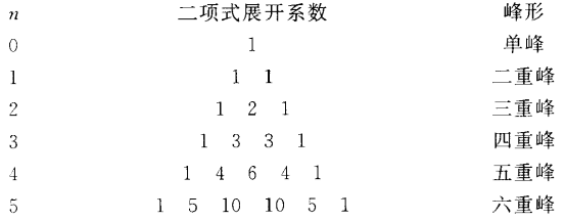
\includegraphics[width=0.7\linewidth]{image/chp6_split}
	\caption{裂分峰的强度比}
	\label{fig:chp6split}
\end{figure}

\subsection{耦合常数}

\begin{definition*}{耦合常数}{}
	耦合常数$J$:谱线裂分所产生的裂距,反映两个核之间的作用力强弱,单位Hz。与两核之间相隔的化学键数目关系很大。在$J$的左上方标以两核相距的化学键数目。
\end{definition*}

\begin{itemize}
	\item $^{2}J$:同碳上的氢,无耦合。不同种磁性核时,有耦合。
	\item $^{3}J$:相邻碳上的氢。如$\ce{H_A-CH2-CH2-H_B}$,$\ce{H_A}$与$\ce{H_B}$的耦合。
	\item $^{4}J$:相隔4个化学键,耦合作用很弱。若$J\neq 0$,则称长程耦合。
\end{itemize}

\section{一级谱图的解析}
%4、熟悉一级谱图的解析。

\subsection{一级谱图}
\begin{itemize}
	\item 满足$(\Delta \nu/J)>6$条件的谱图称为一级谱图。$\Delta \nu$为化学位移之差;$J$为耦合常数。
	\item 相同$\delta$值得几个核对任一另外的核有相同的耦合常数。
	\item (n+1)规律只适用于一级谱图:见\ref{sec:n+1}
\end{itemize}

\subsection{谱图上能获得的主要信息}
\begin{itemize}
	\item 化学位移——判断核所处的\textbf{化学环境};
	\item 耦合裂分——从峰的裂分个数及偶合常数鉴别谱图中相邻的核,以说明分子中基团间的\textbf{空间关系};
	\item 积分线——高度代表了各组峰面积,而峰面积与分子中相应的各种核的数目成正比,通过比较积分线高度可以确定各组核的\textbf{相对数目}。
\end{itemize}

\subsection{常见化合物的质子位移}

\subsubsection{烷基}
对于烷基,$\delta$值一般在0~2 ppm 。
\begin{itemize}
	\item 饱和$\ce{-CH3}$:在高场约0.9ppm出峰,峰强,在连接烷基链时易于辨认。
	\item $\ce{-CH2-}$一般较$\ce{-CH3}$大0.3ppm,$\ce{-CH-}$又较$\ce{-CH2-}$大0.3ppm
\end{itemize}

\begin{figure}
	\centering
	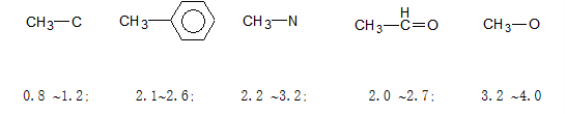
\includegraphics[width=0.7\linewidth]{image/chp6_delta1}
	\caption{甲基}
	\label{fig:chp6delta1}
	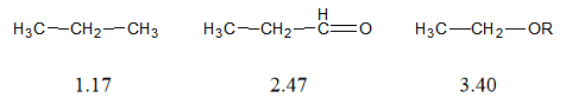
\includegraphics[width=0.7\linewidth]{image/chp6_delta2}
	\caption{亚甲基}
	\label{fig:chp6delta2}
\end{figure}

\subsubsection{烯}
$\delta$值一般在4~7 ppm(6.5 ppm左右较普遍);当双键连有卤素原子时,卤素所连碳上的另一个氢$\delta$最大,即图中的$\delta_{\ce{^{1}H_c}}$最大。

\subsubsection{苯环}
\begin{itemize}
	\item 无取代基时,$\delta_{\ce{^{1}H}}=7.3$ ppm, 单峰
	\item 烃基单取代:如$\ce{-CH3},\ce{-CH2-}$等,一组峰,分辨不开
	\item 活化基团单取代:两组高场峰,邻对位在较高场(无法分辨),间位在较低场
	\item 钝化基团单取代:两组低场峰,间对位在较高场(无法分辨),邻位在较低场
\end{itemize}

\subsubsection{醛基氢}
$\delta$值一般在9~10ppm。

\subsubsection{羧基氢}
$\delta$值一般在12+ppm。

可参考下图:
\begin{figure}[!h]
	\centering
	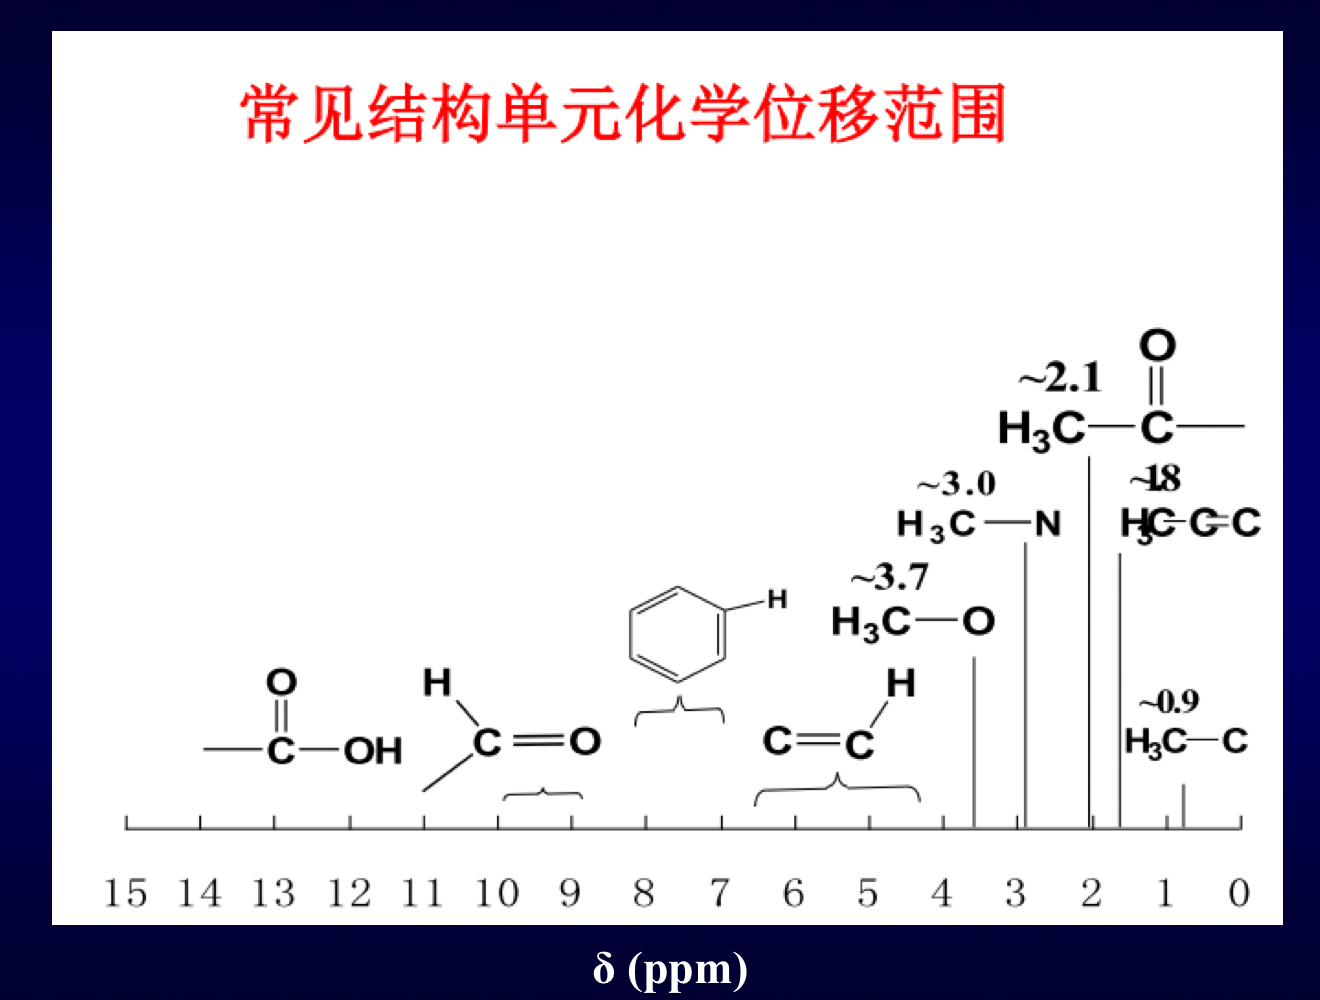
\includegraphics[width=0.6\linewidth]{image/chp6_1HNMR}
%	\caption{}
	\label{fig:chp61hnmr}
\end{figure}


需要说明化学等价的的概念:指同一个碳上的原子($\alpha$位有手性碳的不是)或在分子中处于对称(旋转轴、对称中心、对称面)位置的质子。


\subsection{化学位移的影响因素}
\subsubsection{取代基电负性—诱导效应}
取代基电负性越强,\textbf{吸电子作用越强,价电子偏离质子,屏蔽效应减弱},信号峰在低场出现。

\begin{example}
	相连碳原子的sp杂化。从$\ce{sp^3}$到$\ce{sp^2}$,s电子的成分从25\%增加到33\%,键电子更靠近碳原子,对质子有去屏蔽效应,共振位置移向低场。如图\ref{fig:chp61hnmrx}:
\begin{figure}[!h]
	\centering
	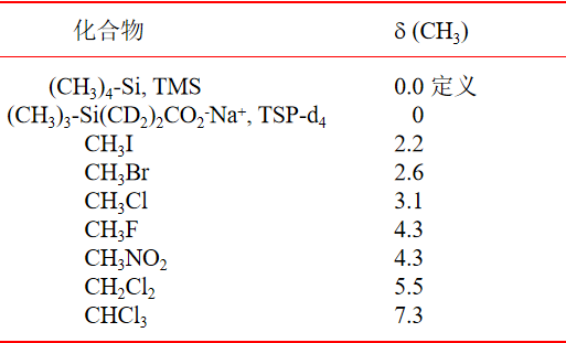
\includegraphics[width=0.5\linewidth]{image/chp6_1HNMR_X}
	\caption{诱导效应的影响}
	\label{fig:chp61hnmrx}
\end{figure}
\end{example}

\subsubsection{环电流效应}
环状共轭体系(4n+2)的离域$\pi$电子产生环电流,环电流产生的磁力线方向在苯环上下方与外磁场磁感应强度方向相反,在苯环侧面方向相同。类似物理中的楞次效应。

结果:环外氢为顺磁效应,去屏蔽,$\delta$增大;环内侧氢为逆磁效应,屏蔽,$\delta$减小。

\begin{example}
18-轮烯:环外氢$\delta$为正;环内侧氢$\delta$为负。

\begin{figure}[!h]
	\centering
	\subfigure[环电流]{
		\begin{minipage}[t]{0.42\linewidth}
			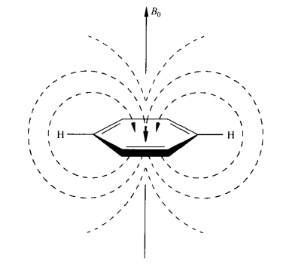
\includegraphics[width=\textwidth]{chp6_benzene}
	\end{minipage}}
	\quad
	\subfigure[18-轮烯]{
		\begin{minipage}[t]{0.42\linewidth}
			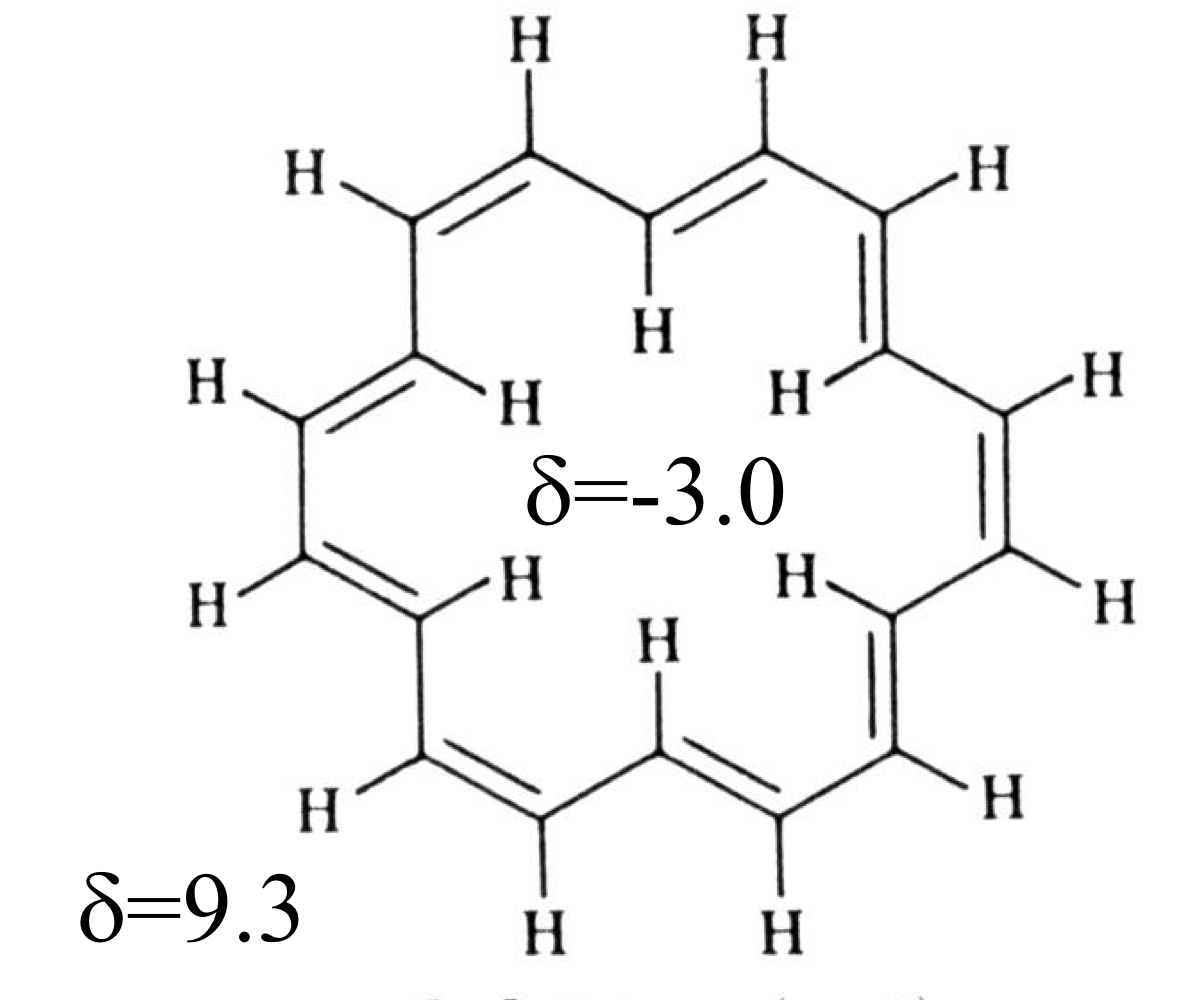
\includegraphics[width=\textwidth]{chp6_18}
	\end{minipage}}
\end{figure}

\end{example}

\subsubsection{相邻键的磁各向异性}
一般的,三键电子云磁感应强度与键轴共线,而双键电子云产生的磁感应强度则与分子平面垂直。
\begin{figure}[!h]
	\centering
	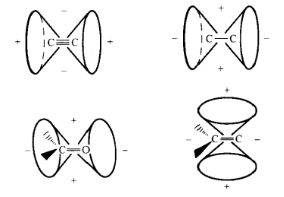
\includegraphics[width=0.6\linewidth]{image/chp6_doubletriplebond}
%	\caption{}
	\label{fig:chp6doubletriplebond}
\end{figure}

\begin{itemize}
	\item 双键C上的氢受去屏蔽作用,$\delta$值高于饱和C;
	\item 叁键C上的氢受屏蔽作用,$\delta$减小。
\end{itemize}

\subsubsection{其他作用}
电偶极和范德华力,介质,氢键等。

\section{核磁共振波谱仪}
%5、了解核磁共振波谱仪的基本组成及各部分功能,了解样品的制备。

\subsection{基本组成及功能}
\subsubsection{外加磁场}
强弱的表示:磁场强度$B_0$,单位:$\mathrm{T}$。
不过习惯用氢核的共振频率来表示。
	如100M的仪器,$B_0=2.35\mathrm{T}$。

要求:强而稳定、均匀

磁铁:分为永久磁铁、电磁铁和超导磁铁。

性能影响因素:
\begin{itemize}
	\item 磁场强度越强,低能级上核的数目越多,灵敏度越高。
	\item 磁场越强,以频率表示的化学位移越大,分辨率越高。
	\item 磁场的均一性越好,分辨率越高。
\end{itemize}

\subsubsection{探头}
呈圆柱形,安装于在磁体中心。作用:对样品管发射脉冲电磁波,检测核磁共振信号。

分类:
\begin{itemize}
	\item 产生固定频率的探头
	\begin{itemize}
		\item 双核探头($\ce{^{1}H,^{13}C}$)
		\item 四核探头($\ce{^{1}H,^{13}C,^{15}N,^{31}P}$)
	\end{itemize}
	\item 频率连续可调探头:如$\ce{^{15}N}$和$\ce{^{31}P}$。
\end{itemize}

\subsubsection{高频电磁波发生器及接受器}
\begin{itemize}
	\item 连续波NMR仪器(CW-NMR)——最简单
	\begin{itemize}
		\item 有两种扫描方式。扫频方式:固定$B_0$,扫描电磁波频率$\nu$;扫场方式:固定$\nu$,扫描磁场强度$B_0$。
		\item 不足:连续变化一个参数使不同基团的核依次满足共振条件,任一瞬间只有一种原子核处于共振状态,其它核处于等待状态。样品利用率低,灵敏度低,分辨率低。
	\end{itemize}
	\item 傅里叶变换NMR(FT-NMR)
	\begin{itemize}
		\item 磁场强,产生强而短的脉冲(高频脉冲)。在这一脉冲下,所有的核都发生共振。脉冲停止后,这些核都产生相应的核磁共振信号。这些信号含多种频率,总信号是多种频率信号的叠加,这些信号以时间为变量,也是随时间衰减的。因此,信号是时间的函数(时域谱),通过FT转换变为频域谱。
		\item 优点:所有的核同时共振;灵敏度高,样品用量少;测定时间短,可多次去平均能降低噪声。
	\end{itemize}
\end{itemize}

\subsubsection{数据处理及记录部分}

\subsection{样品制备技术}
\begin{itemize}
	\item 样品要制成粘度不高的液态:2-15\%的溶液
	\item NMR溶剂不应含氢,可用卤化或氘代溶剂,如$\ce{CDCl3, C6D6}$等。
\end{itemize}


\section{$\ce{^{13}C}$谱}
%6、简要了解碳-13谱,和氢谱相比,有什么特点?
$\ce{^{13}C}$的自然丰度约为1\%,即样品中所有$\ce{C}$只约有1\%是$\ce{^{13}C}$。由于分子数是巨大的,而原子的分布是随机的,所以可以认为分子中每个碳原子都有1\%几率是$\ce{^{13}C}$,这样就可测得代表整个分子的$\ce{^{13}C}$MR。由于$\ce{^{13}C}$自然丰度低,$\ce{^{13}C}$MR的相对灵敏度仅为氢谱的1/5600。
特点:
\begin{itemize}
	\item 碳的δ值范围0~230ppm。因为$\ce{C}$外层$\ce{p}$电子云密度变化范围大,对$\ce{C}$核的屏蔽效应变化范围也大。因此其信号不像PMR那样容易重叠,往往分子中有几个不同类$\ce{C}$,就有几组峰,能直接提供有机物碳骨架的信息。
	\item $\ce{^{13}C}$MR没有积分曲线。峰的强度与$\ce{C}$个数无关,却正比于碳上所连的$\ce{H}$数。在$\ce{^{13}C}$MR中,只提供有几类$\ce{C}$的信息,没有提供各类$\ce{C}$的相对比例。
	\item $\ce{^{13}C}$和$\ce{H}$有耦合:耦合的碳谱很乱,很难解析必须把$\ce{^{13}C}$与$\ce{^{1}H}$的偶合裂分峰去掉才行。(可以采用不同的技术进行测定)
\end{itemize}


\section{解谱例题}

\begin{example}
	某化合物分子式为$\ce{C9H12O}$,其$\ce{^{1}H}$ NMR谱如下,推测该化合物的结构。
	
	\begin{figure}[!h]
		\centering
		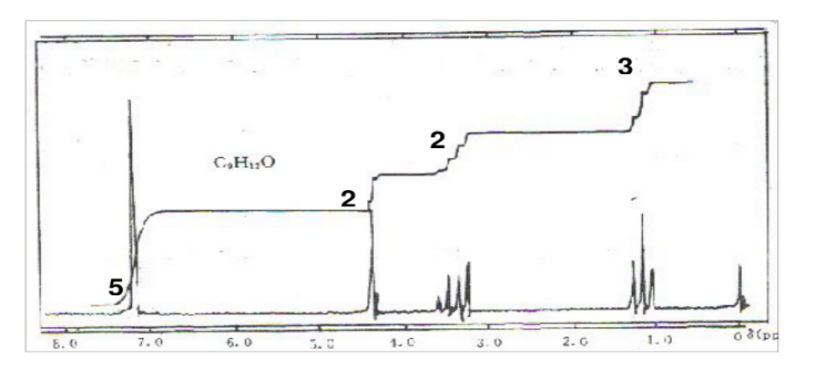
\includegraphics[width=0.9\linewidth]{image/chp6_example1}
%		\caption{}
		\label{fig:chp6example1}
	\end{figure}

	\solve
	不饱和度为4,$\delta=7.2$左右的是单取代苯的峰,所以没有其他双键和环,又无醇羟基峰,考虑醚类;3氢的三重峰和2氢的四重峰对应乙基,后者化学位移大,可能与氧相连;剩下的2氢单峰化学位移更大,可能还和苯环相连。综上,最可能是苯甲醇乙醇醚。
	\begin{figure}[!h]
		\centering
		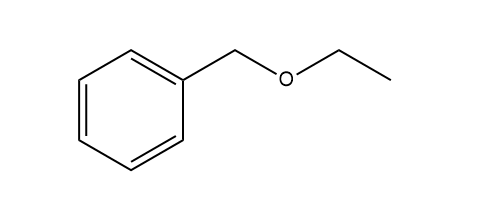
\includegraphics[width=0.6\linewidth]{image/chp6_answer1}
%		\caption{}
		\label{fig:chp6answer1}
	\end{figure}
\end{example}

\begin{example}
	某化合物分子式为$\ce{C8H8O2}$,其$\ce{^{1}H}$ NMR谱如下,推测该化合物的结构。
	
	\begin{figure}[!h]
		\centering
		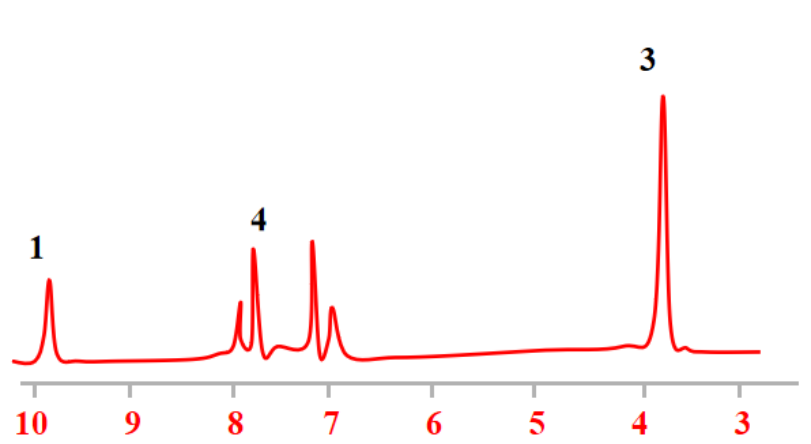
\includegraphics[width=0.7\linewidth]{image/chp6_example2}
%		\caption{}
		\label{fig:chp6example2}
	\end{figure}
	
	\solve	
	不饱和度为5,$\delta=7\sim 8$是芳环上氢,四个峰对位取代;$\delta=9.87$是醛基上氢,低场;$\delta=3.87$是$\ce{-CH3}$峰,向低场位移,与电负性基团相连,所以可能的结构是
	
	\begin{figure}[!h]
		\centering
		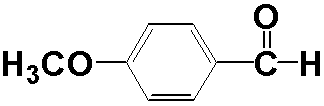
\includegraphics[width=0.5\linewidth]{image/chp6_answer2}
%		\caption{}
		\label{fig:chp6answer2}
	\end{figure}
\end{example}
\end{document}